% Put this in the LaTeX preamble:
% \graphicspath{{thesis_outputs/figures/}{thesis_outputs/tables/}}

% Descriptive statistics:
\begin{table}
\caption{Descriptive statistics of the main variables}
\label{tab:descriptive}
\begin{tabular}{lrrrrrr}
\toprule
Variable & Observations & Mean & Std. Dev. & Min & Median & Max \\
\midrule
$\ln Y$ & 1170 & 7.597000 & 0.527000 & 5.520000 & 7.580000 & 8.805000 \\
$\ln Y_{t-1}$ & 1099 & 7.578000 & 0.524000 & 5.520000 & 7.566000 & 8.805000 \\
$\ln A$ & 1170 & 5.326000 & 2.019000 & -4.828000 & 5.491000 & 8.244000 \\
Growing-season temperature & 1170 & 13.979000 & 3.613000 & 3.140000 & 14.237000 & 22.884000 \\
Growing-season precipitation & 1170 & 388.027000 & 159.334000 & 66.357000 & 376.092000 & 1073.661000 \\
SPI & 1170 & 0.254000 & 0.678000 & -2.126000 & 0.351000 & 2.029000 \\
SPEI & 1170 & 0.254000 & 1.426000 & -4.398000 & 0.361000 & 4.225000 \\
$\ln Sub$ & 529 & 22.762000 & 6.291000 & 4.094000 & 25.118000 & 26.407000 \\
$\ln Sub/A$ & 529 & 17.306000 & 6.610000 & -2.503000 & 19.088000 & 31.116000 \\
\bottomrule
\end{tabular}
\end{table}


% Model comparison:
\begin{table}
\caption{Model comparison summary}
\label{tab:model_comparison}
\begin{tabular}{llrrrrrrrrl}
\toprule
Model & Purpose & N & R2_within & R2_between & R2_overall & RMSE & MAE & CV_R2_mean & CV_R2_std & Main finding \\
\midrule
FE_baseline & Average climate relationship & 521 & 0.138900 & -13.086000 & -8.762000 & NaN & NaN & NaN & NaN &  \\
FE_nonlinear & Nonlinear climate response & 521 & -0.188700 & -10.601700 & -7.089900 & NaN & NaN & NaN & NaN & Tests quadratic terms of temperature, SPI and SPEI \\
FE_post2014_interactions & Change in climate sensitivity after 2014 & 521 & 0.138900 & -13.086000 & -8.762000 & NaN & NaN & NaN & NaN & Post-2014 climate interaction specification \\
SAR_style & Spatial correlation in production & 490 & 0.257600 & -1.728700 & -0.913100 & NaN & NaN & NaN & NaN & Spatial lag of production included \\
SDM_style & Spatial Durbin robustness check & 490 & 0.482800 & -2.255900 & -1.245500 & NaN & NaN & NaN & NaN & Spatial lag of production and spatially lagged covariates included \\
Panel_ARDL_style & Dynamic lagged climate relationships & 364 & -0.051900 & -2.182300 & -1.788500 & NaN & NaN & NaN & NaN & Lagged climate variables included \\
RF_with_lag & Prediction & 124 & NaN & NaN & 0.533200 & 0.273200 & 0.192900 & 0.713800 & 0.089200 & Lagged production dominates \\
RF_without_lag & Prediction without historical production & 124 & NaN & NaN & -0.100000 & 0.419400 & 0.312300 & 0.260800 & 0.246800 & Climate variables become central predictors \\
\bottomrule
\end{tabular}
\end{table}


% Suggested figure calls:
\begin{figure}[H]
\centering

\includegraphics[width=0.85\textwidth]{fig1_climate_data_workflow.png}
\caption{Construction of climate variables and assembly of the panel dataset}
\end{figure}

\begin{figure}[H]
\centering
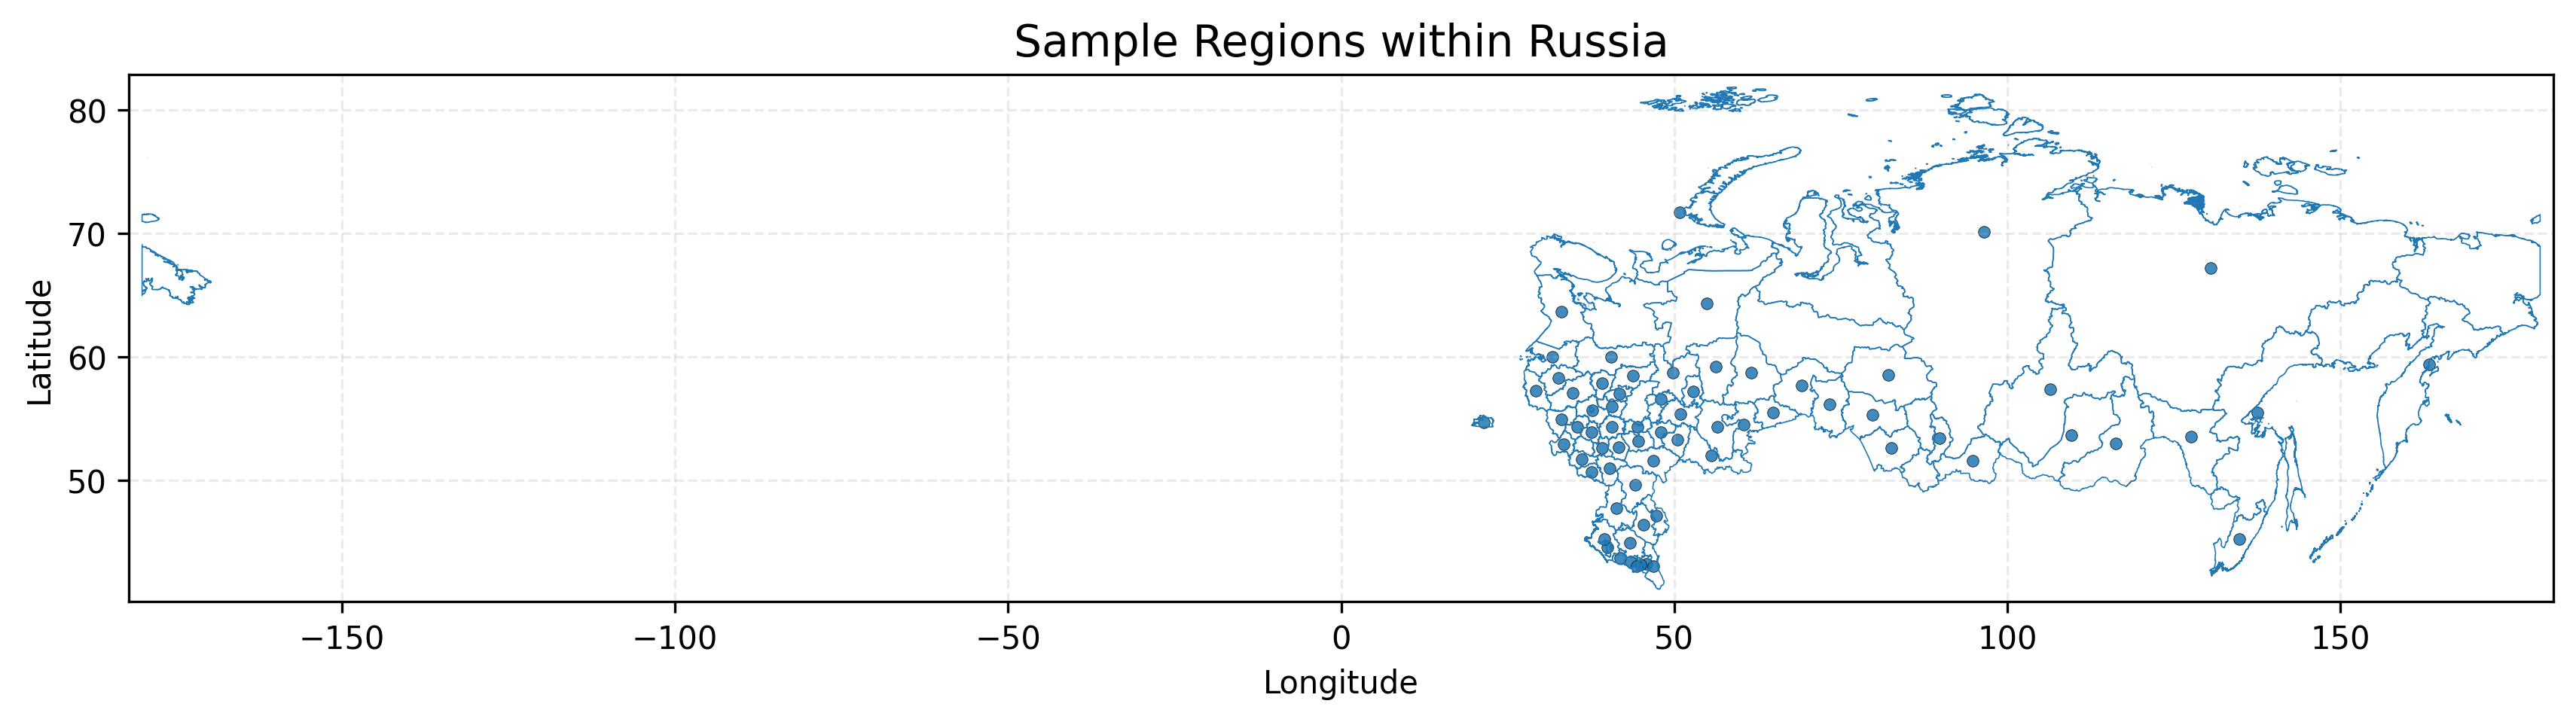
\includegraphics[width=0.90\textwidth]{sample_regions_map.png}
\caption{Outline of Russia and spatial distribution of sample regions}
\end{figure}

\begin{figure}[H]
\centering
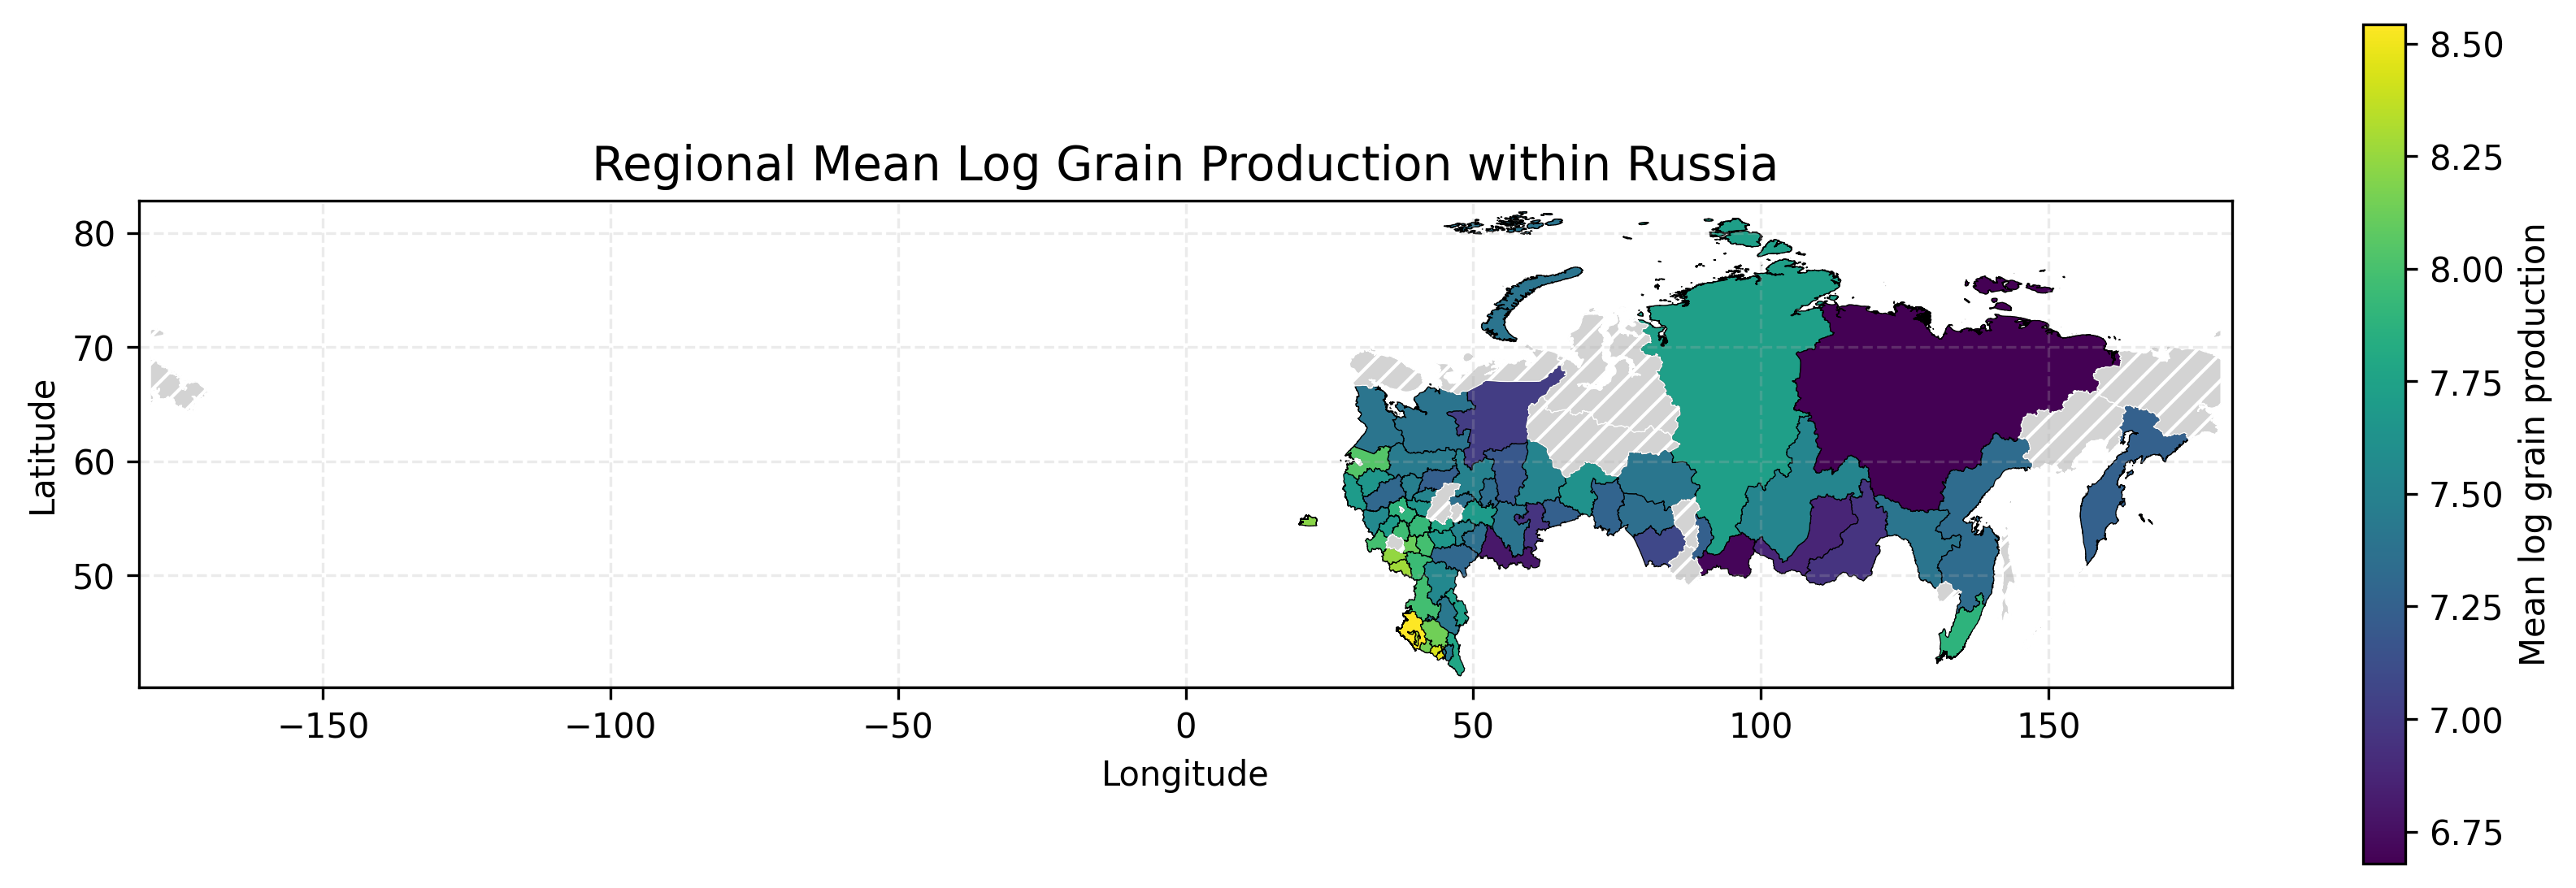
\includegraphics[width=0.90\textwidth]{mean_log_yield_map.png}
\caption{Spatial distribution of average log grain production across Russian regions}
\end{figure}

\begin{figure}[H]
\centering
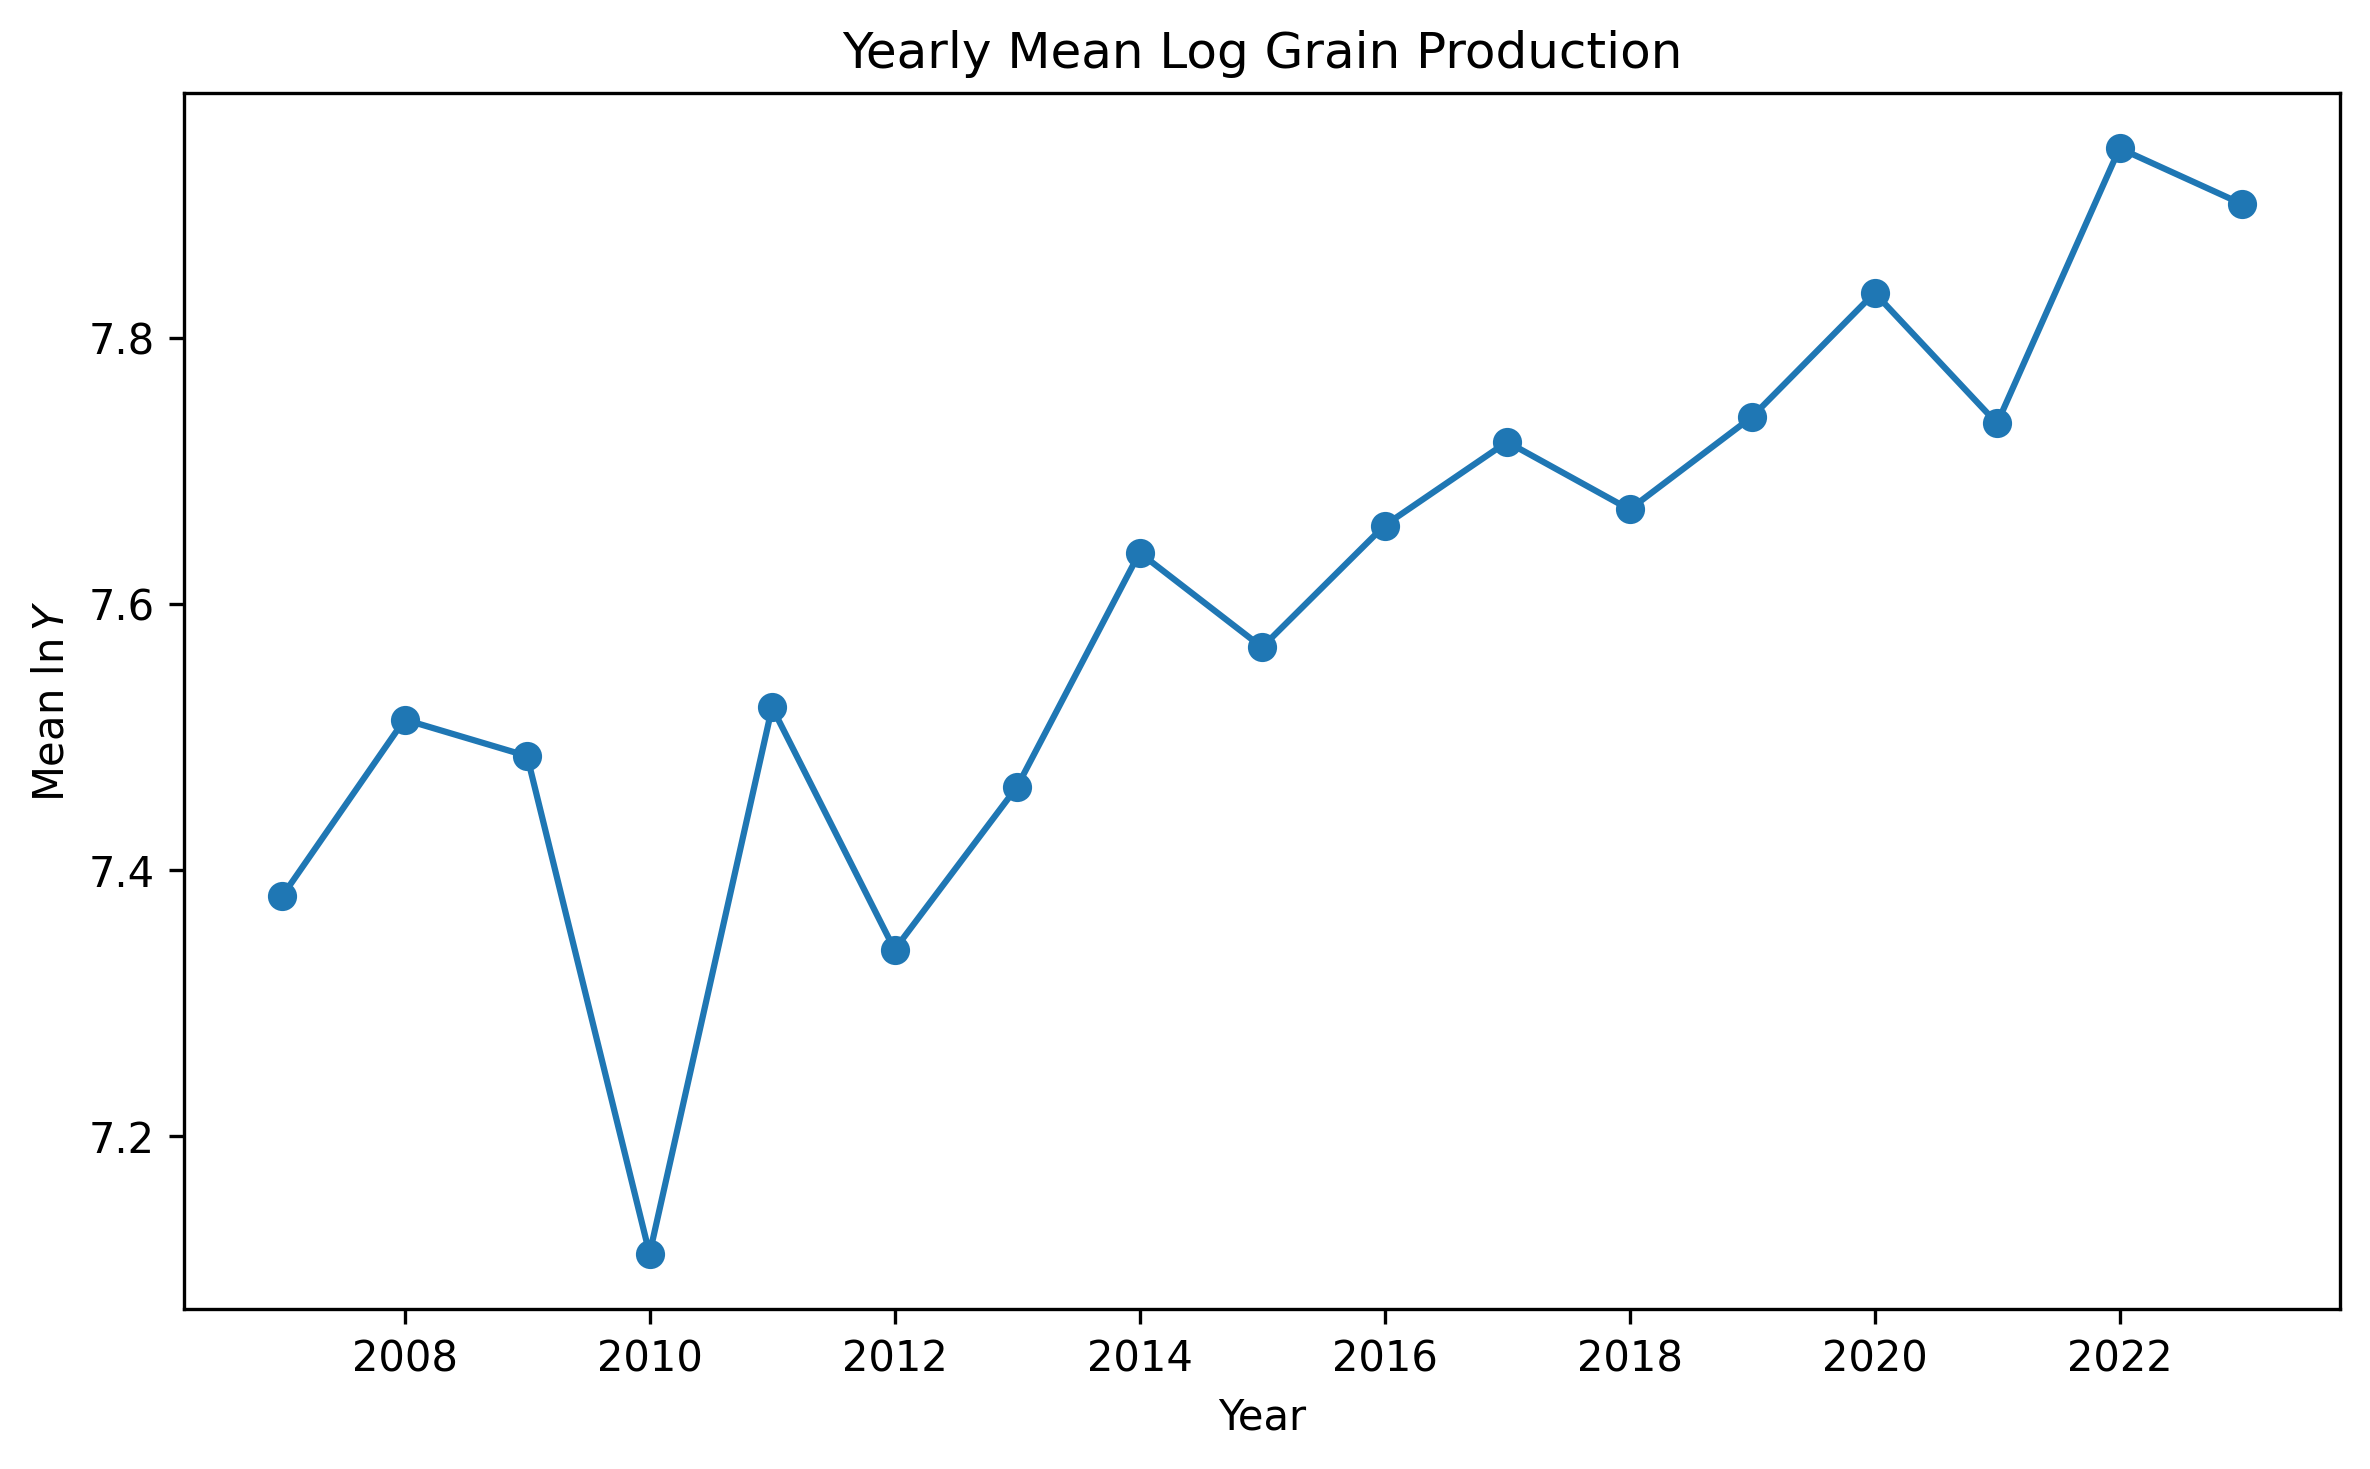
\includegraphics[width=0.75\textwidth]{yearly_mean_log_yield.png}
\caption{Annual changes in regional average log grain production}
\end{figure}

\begin{figure}[H]
\centering
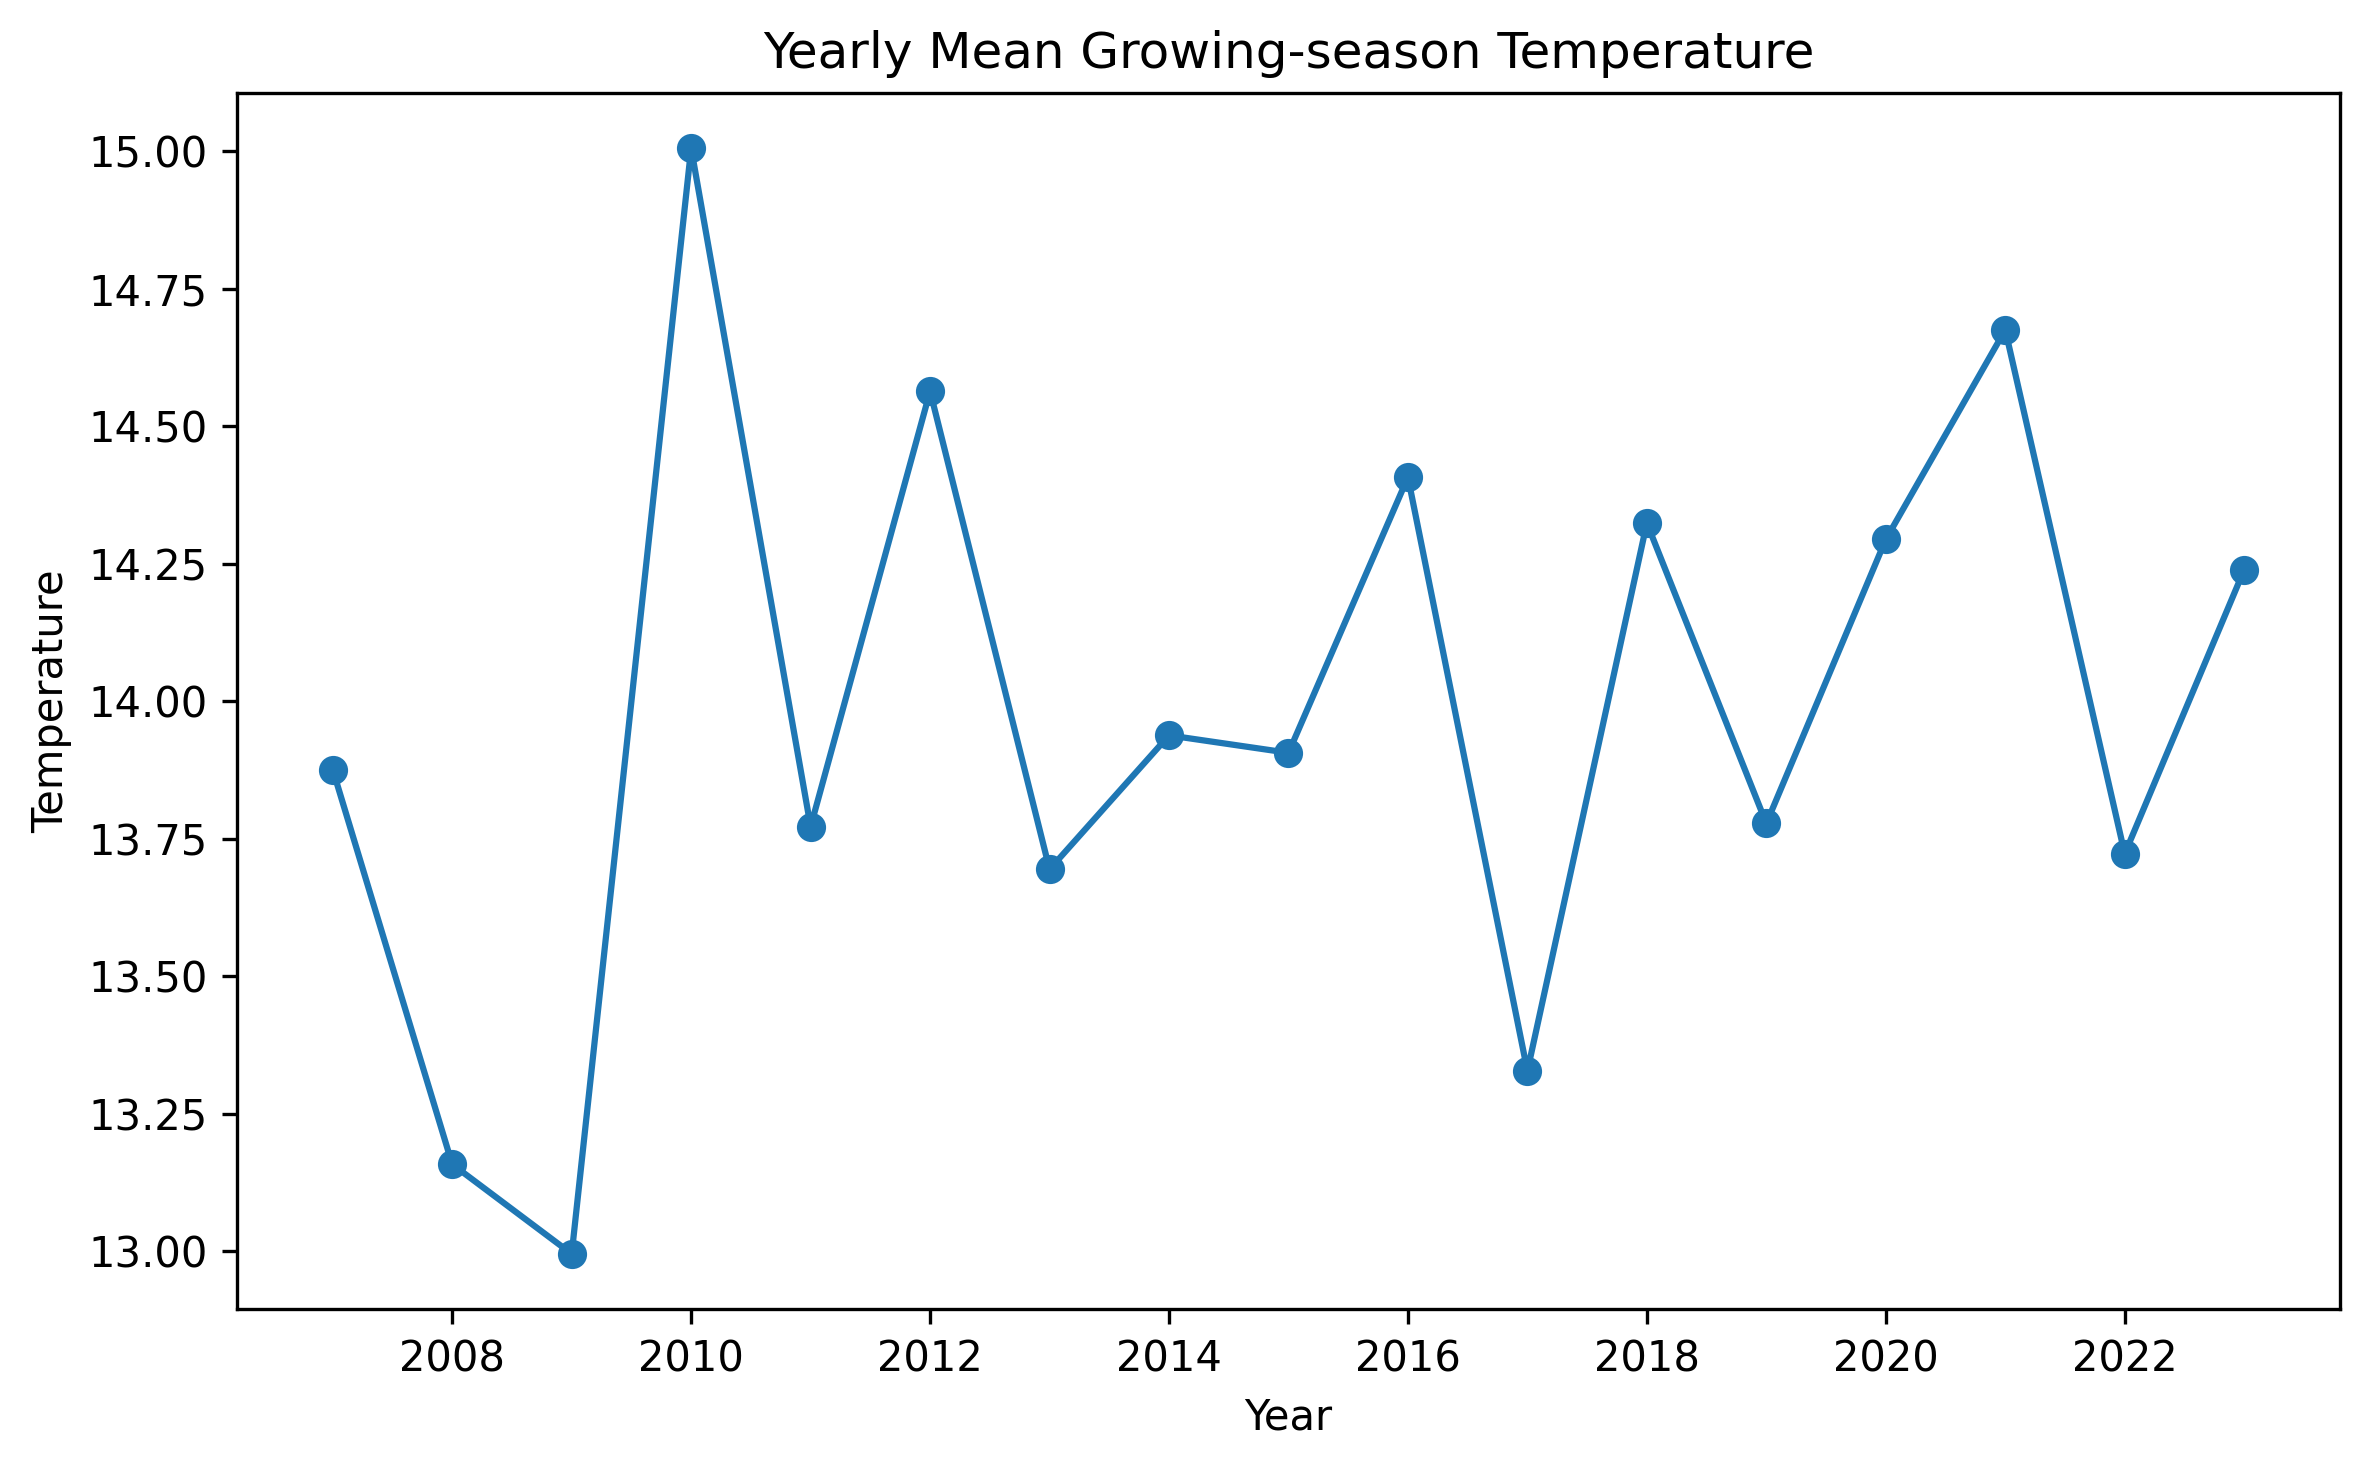
\includegraphics[width=0.75\textwidth]{yearly_mean_temperature.png}
\caption{Annual changes in growing-season average temperature}
\end{figure}

\begin{figure}[H]
\centering
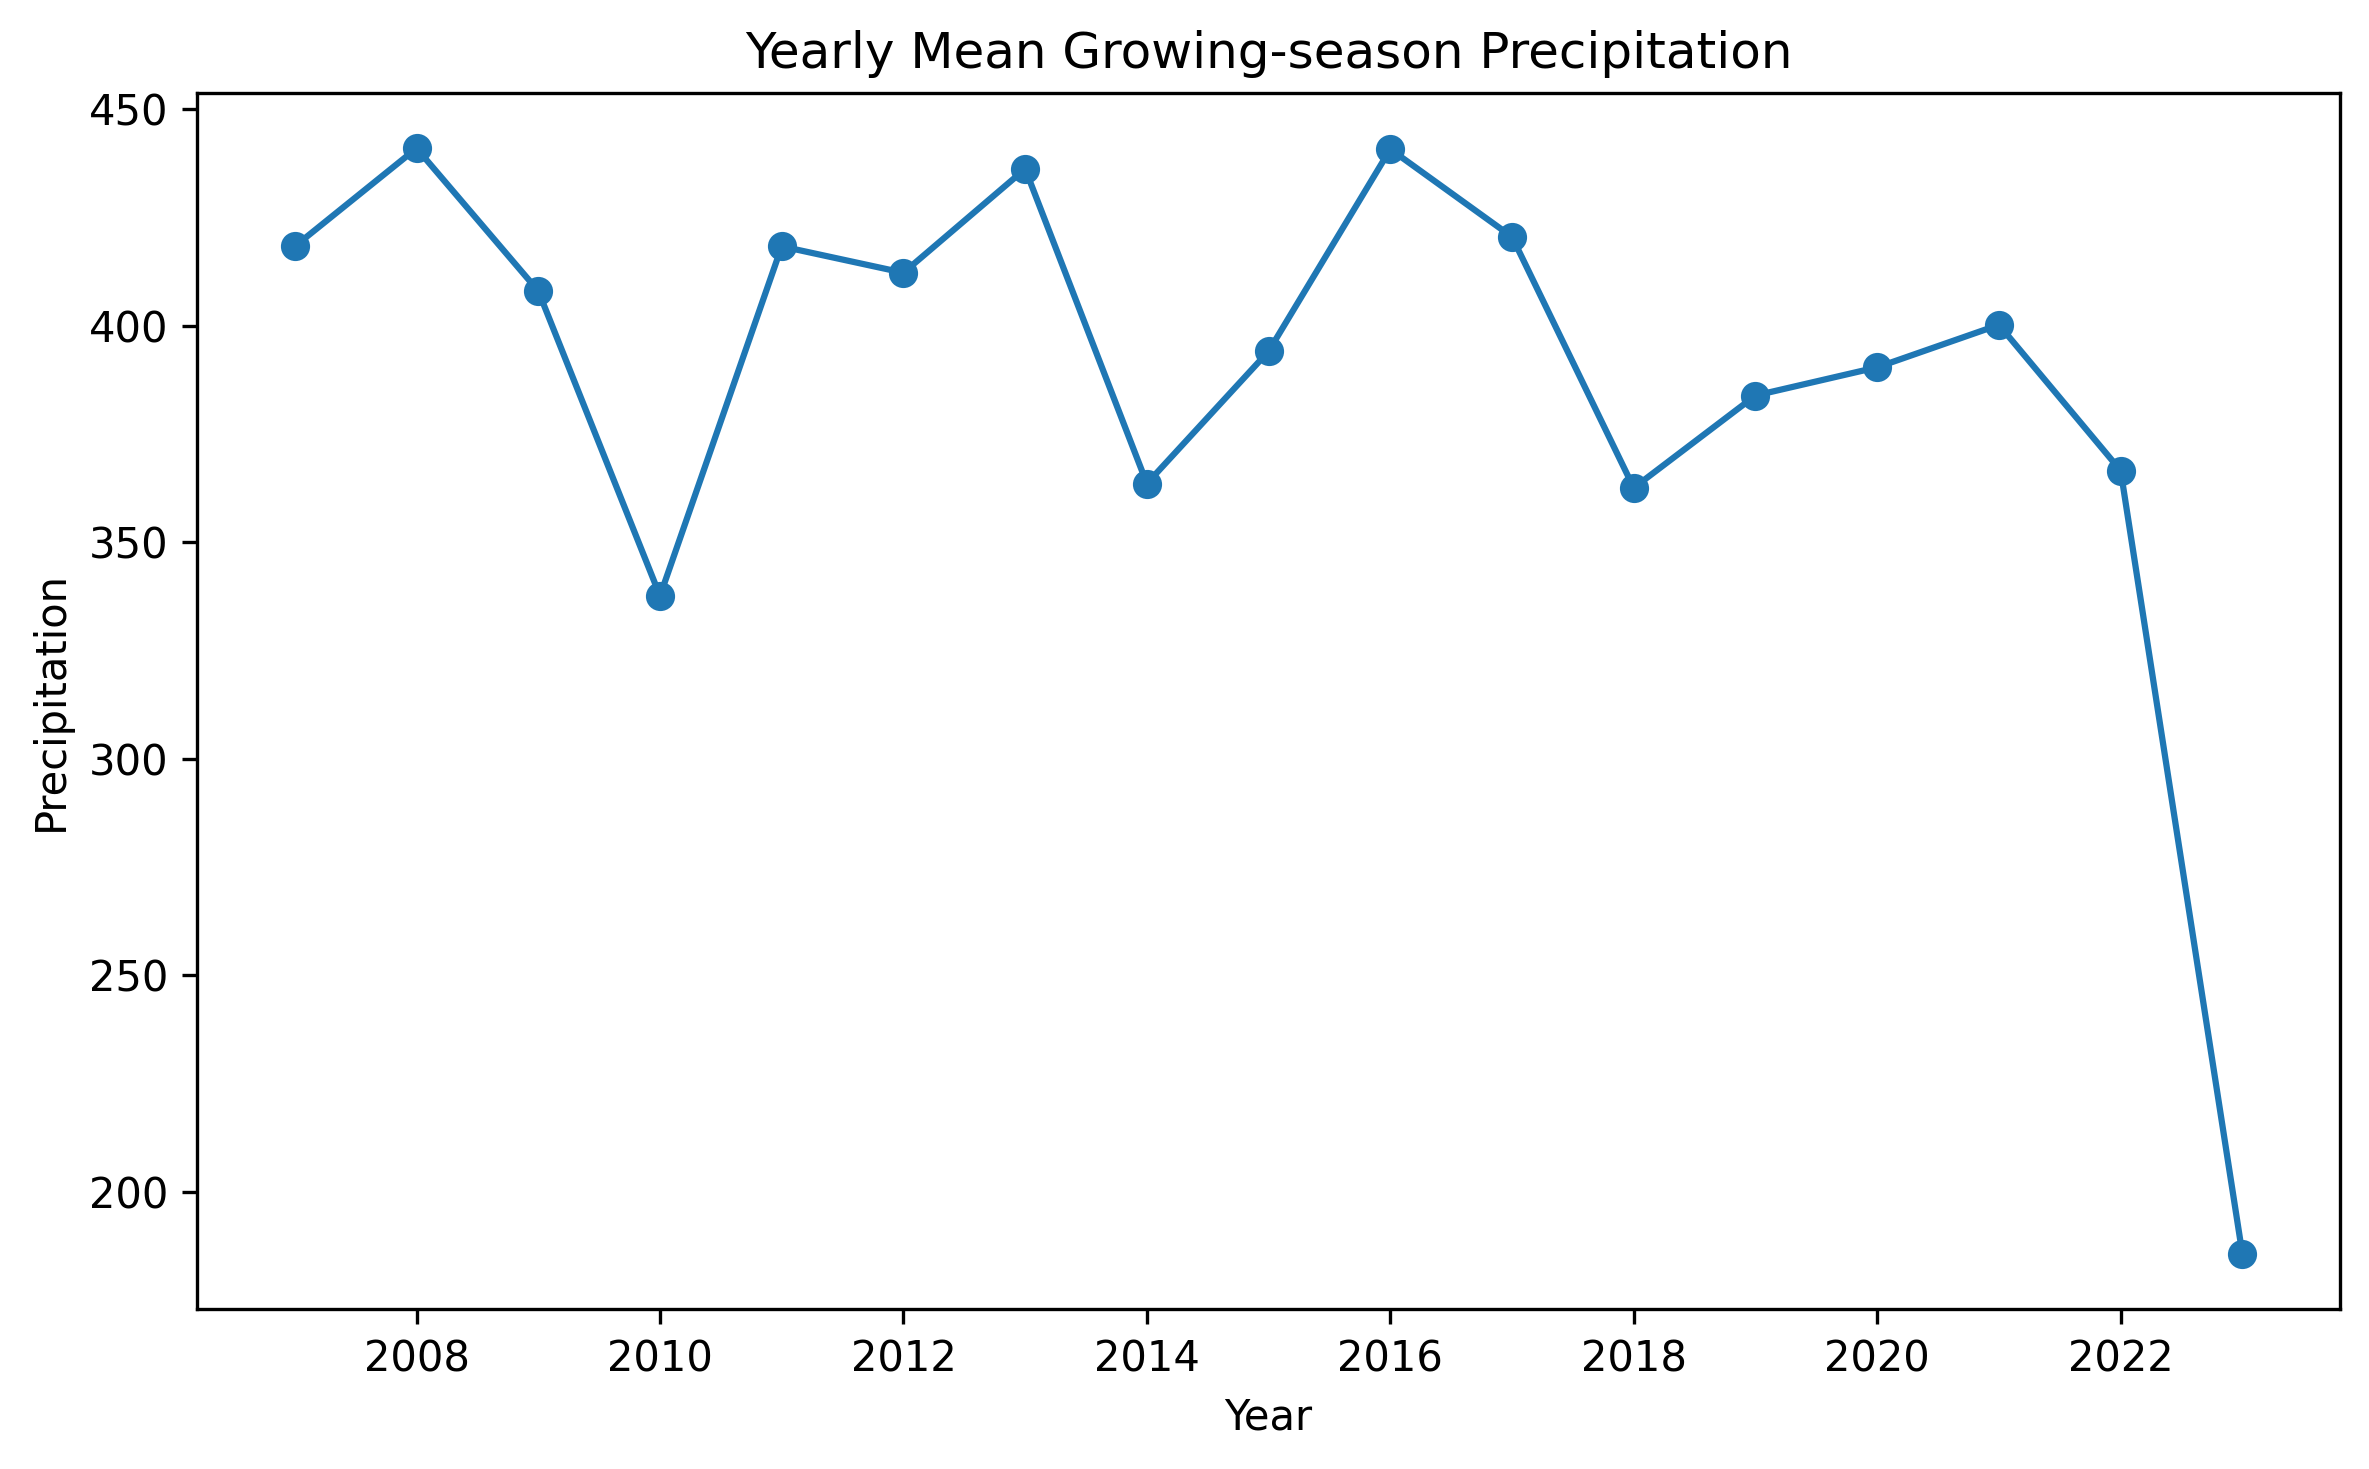
\includegraphics[width=0.75\textwidth]{yearly_mean_precipitation.png}
\caption{Annual changes in growing-season cumulative precipitation}
\end{figure}

\begin{figure}[H]
\centering
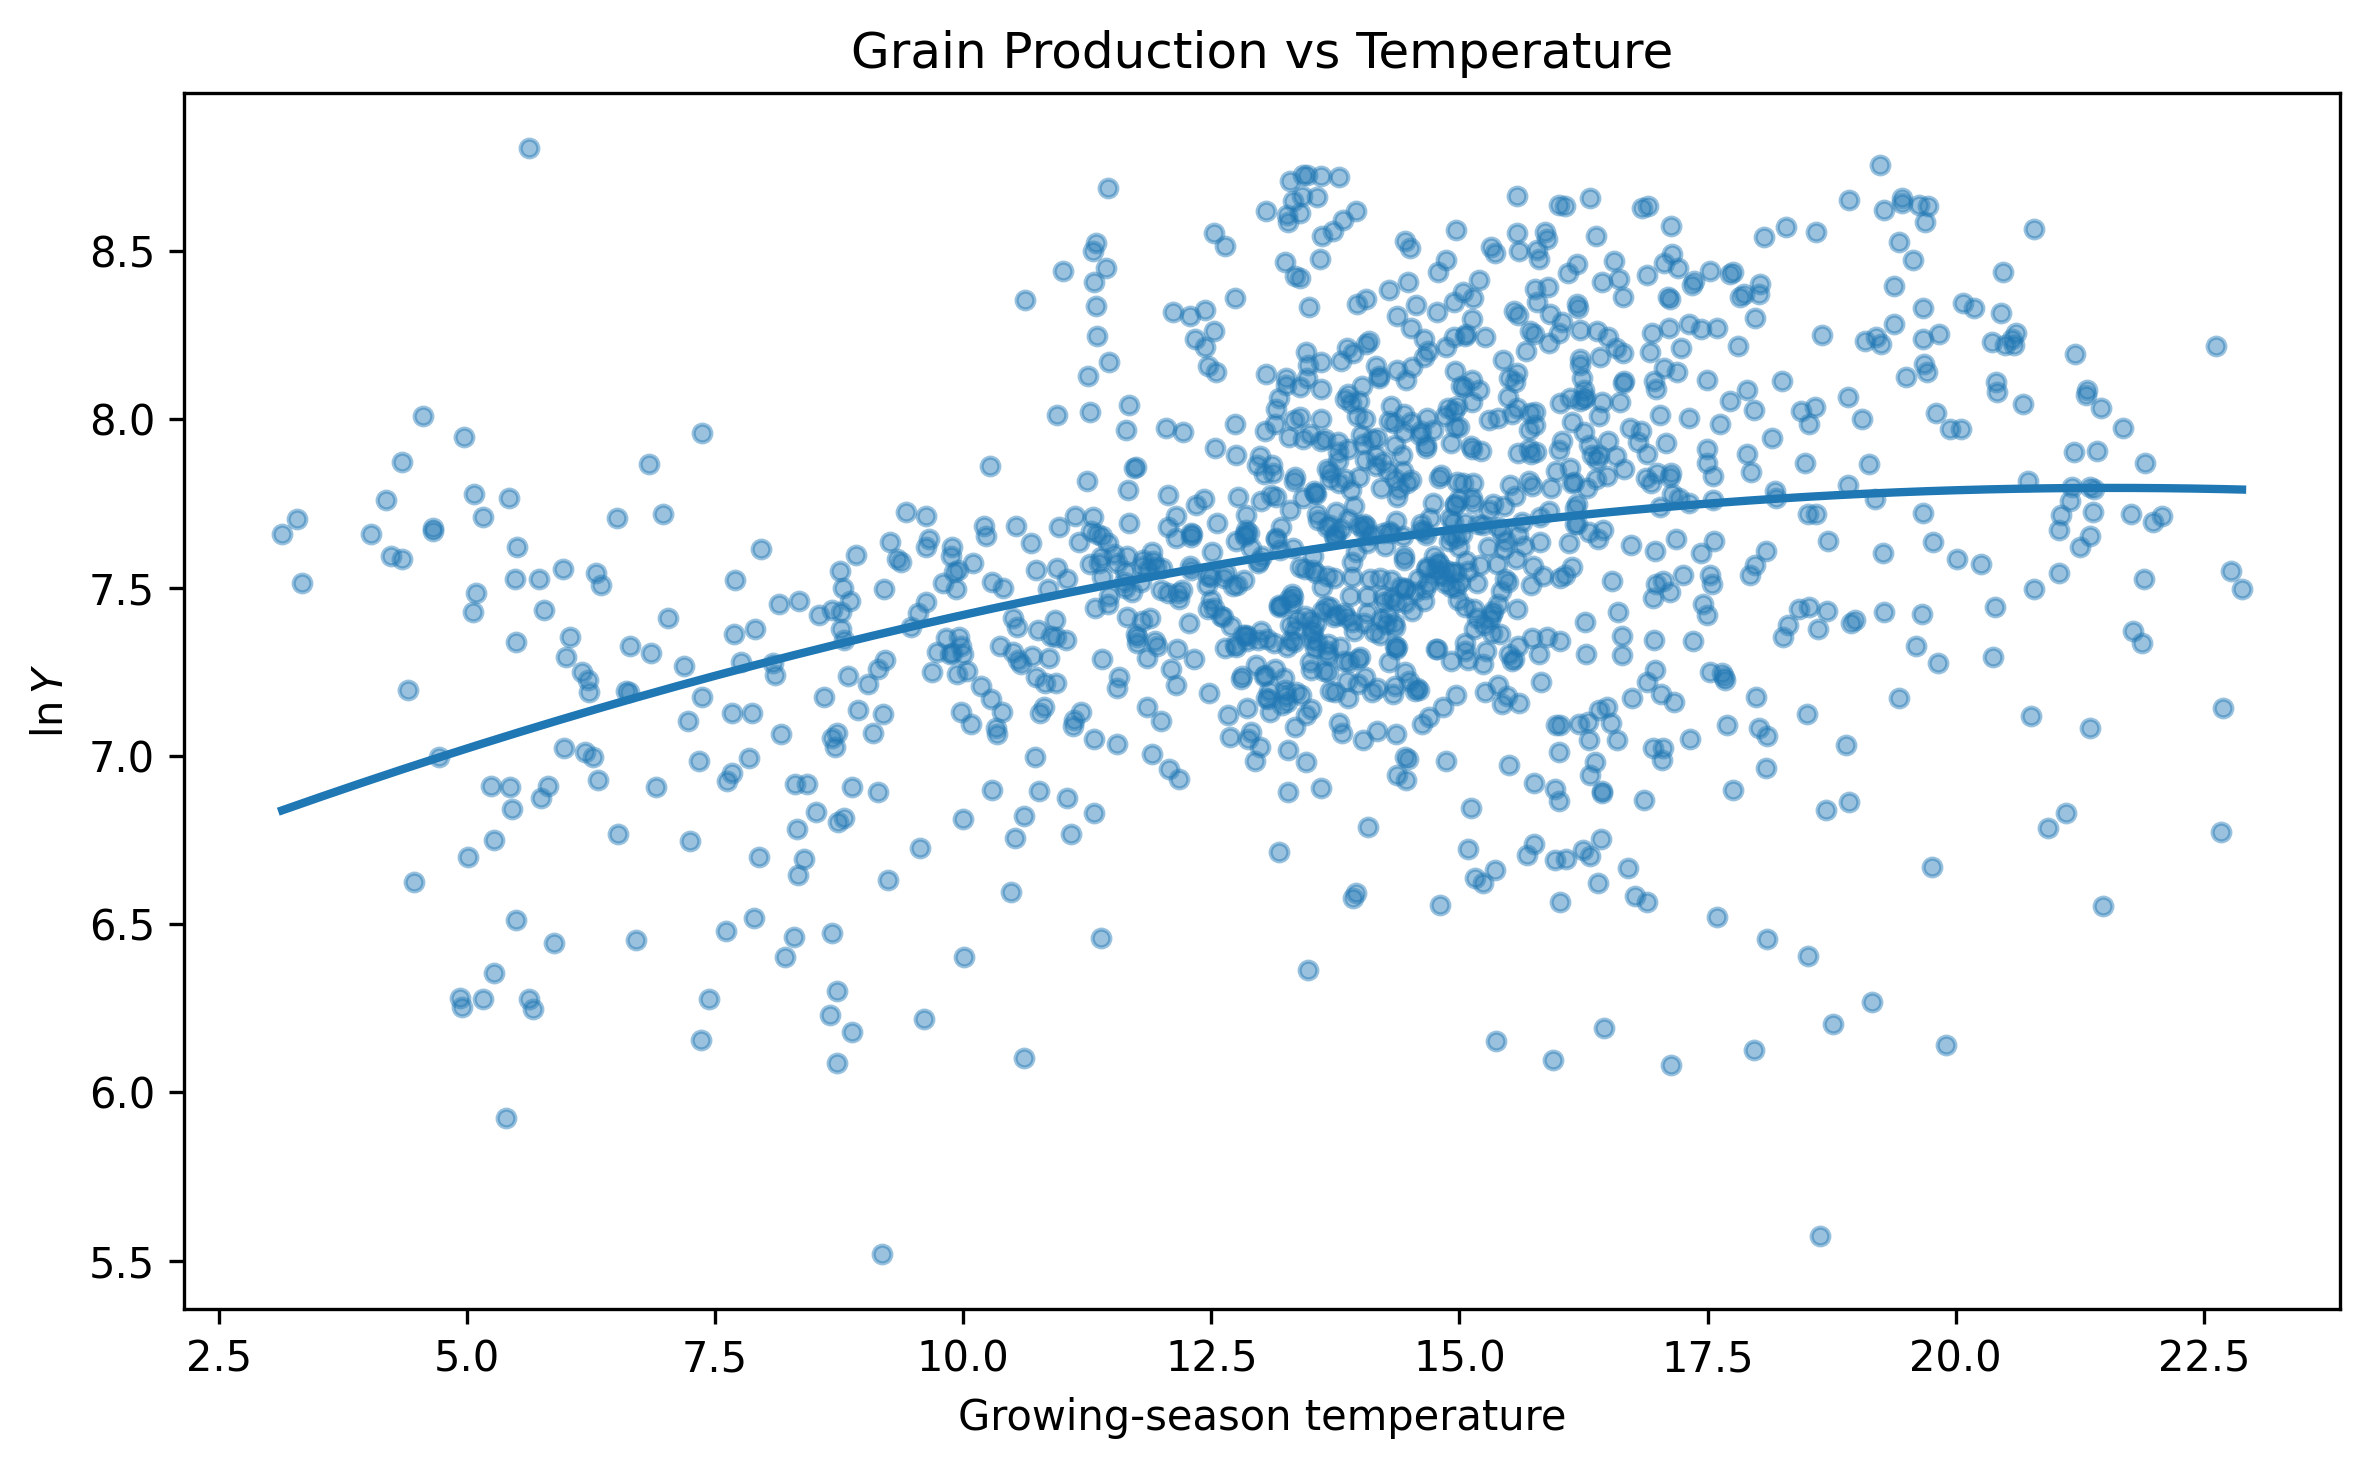
\includegraphics[width=0.75\textwidth]{temp_quadratic_fit.png}
\caption{Nonlinear relationship between growing-season average temperature and log grain production}
\end{figure}

\begin{figure}[H]
\centering
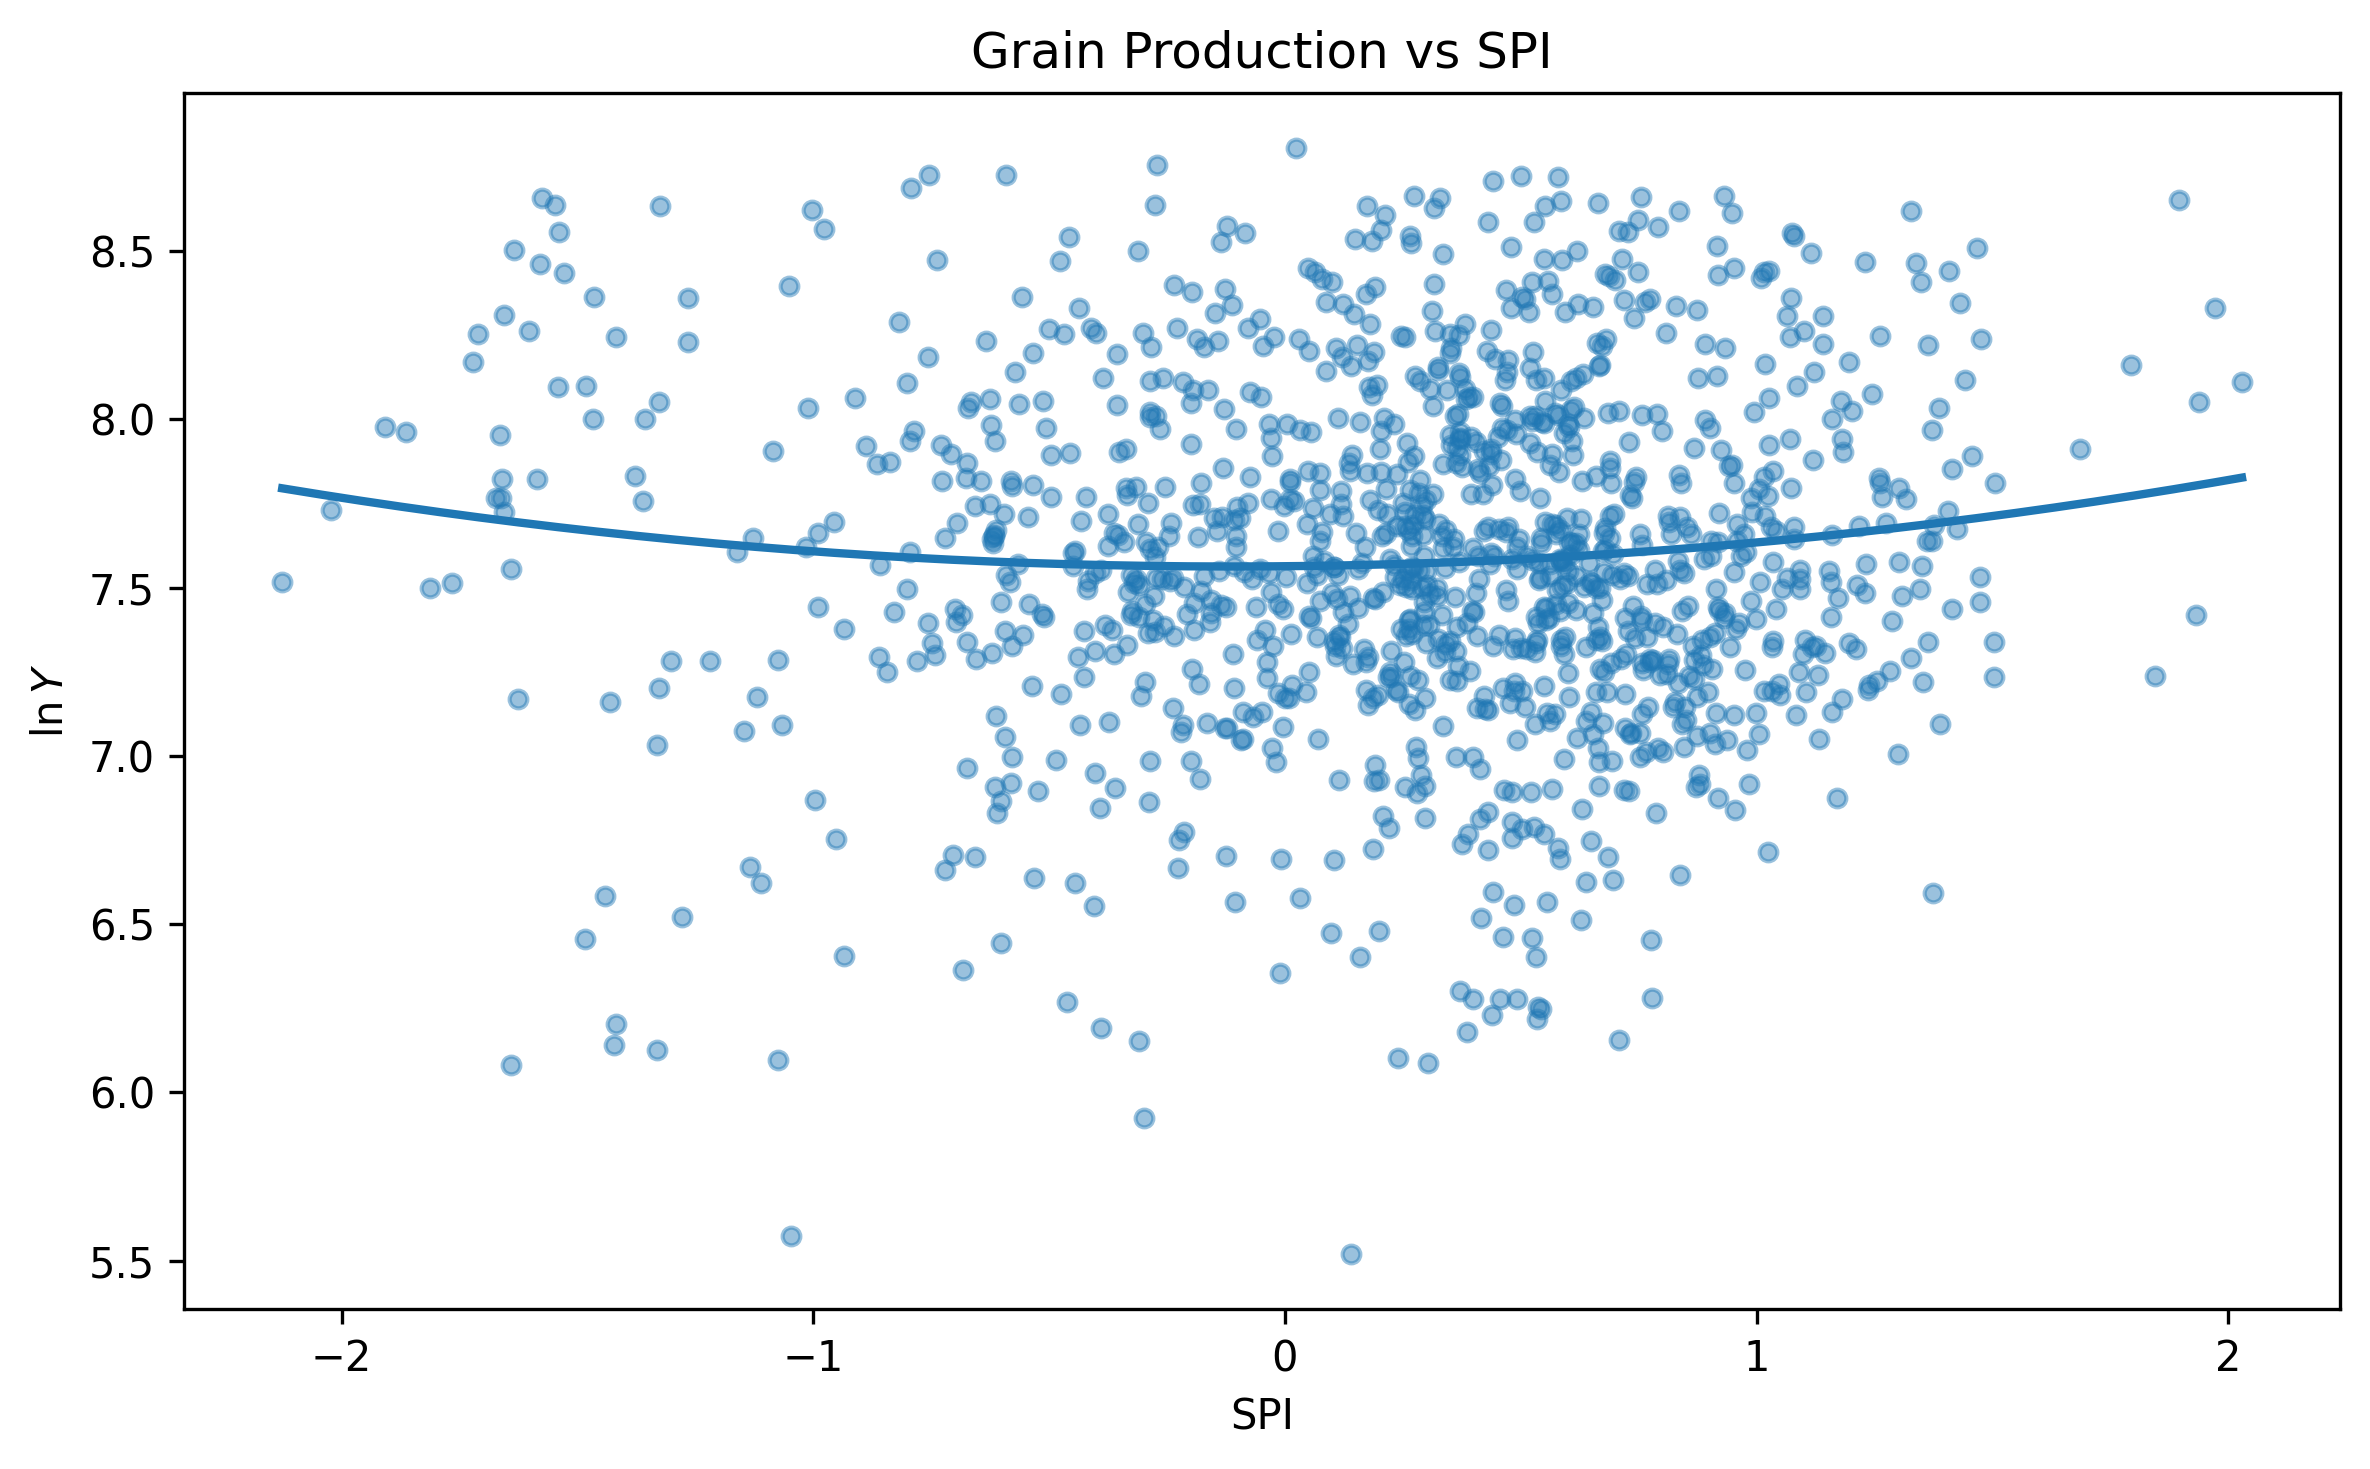
\includegraphics[width=0.75\textwidth]{spi_quadratic_fit.png}
\caption{Nonlinear relationship between SPI and log grain production}
\end{figure}

\begin{figure}[H]
\centering
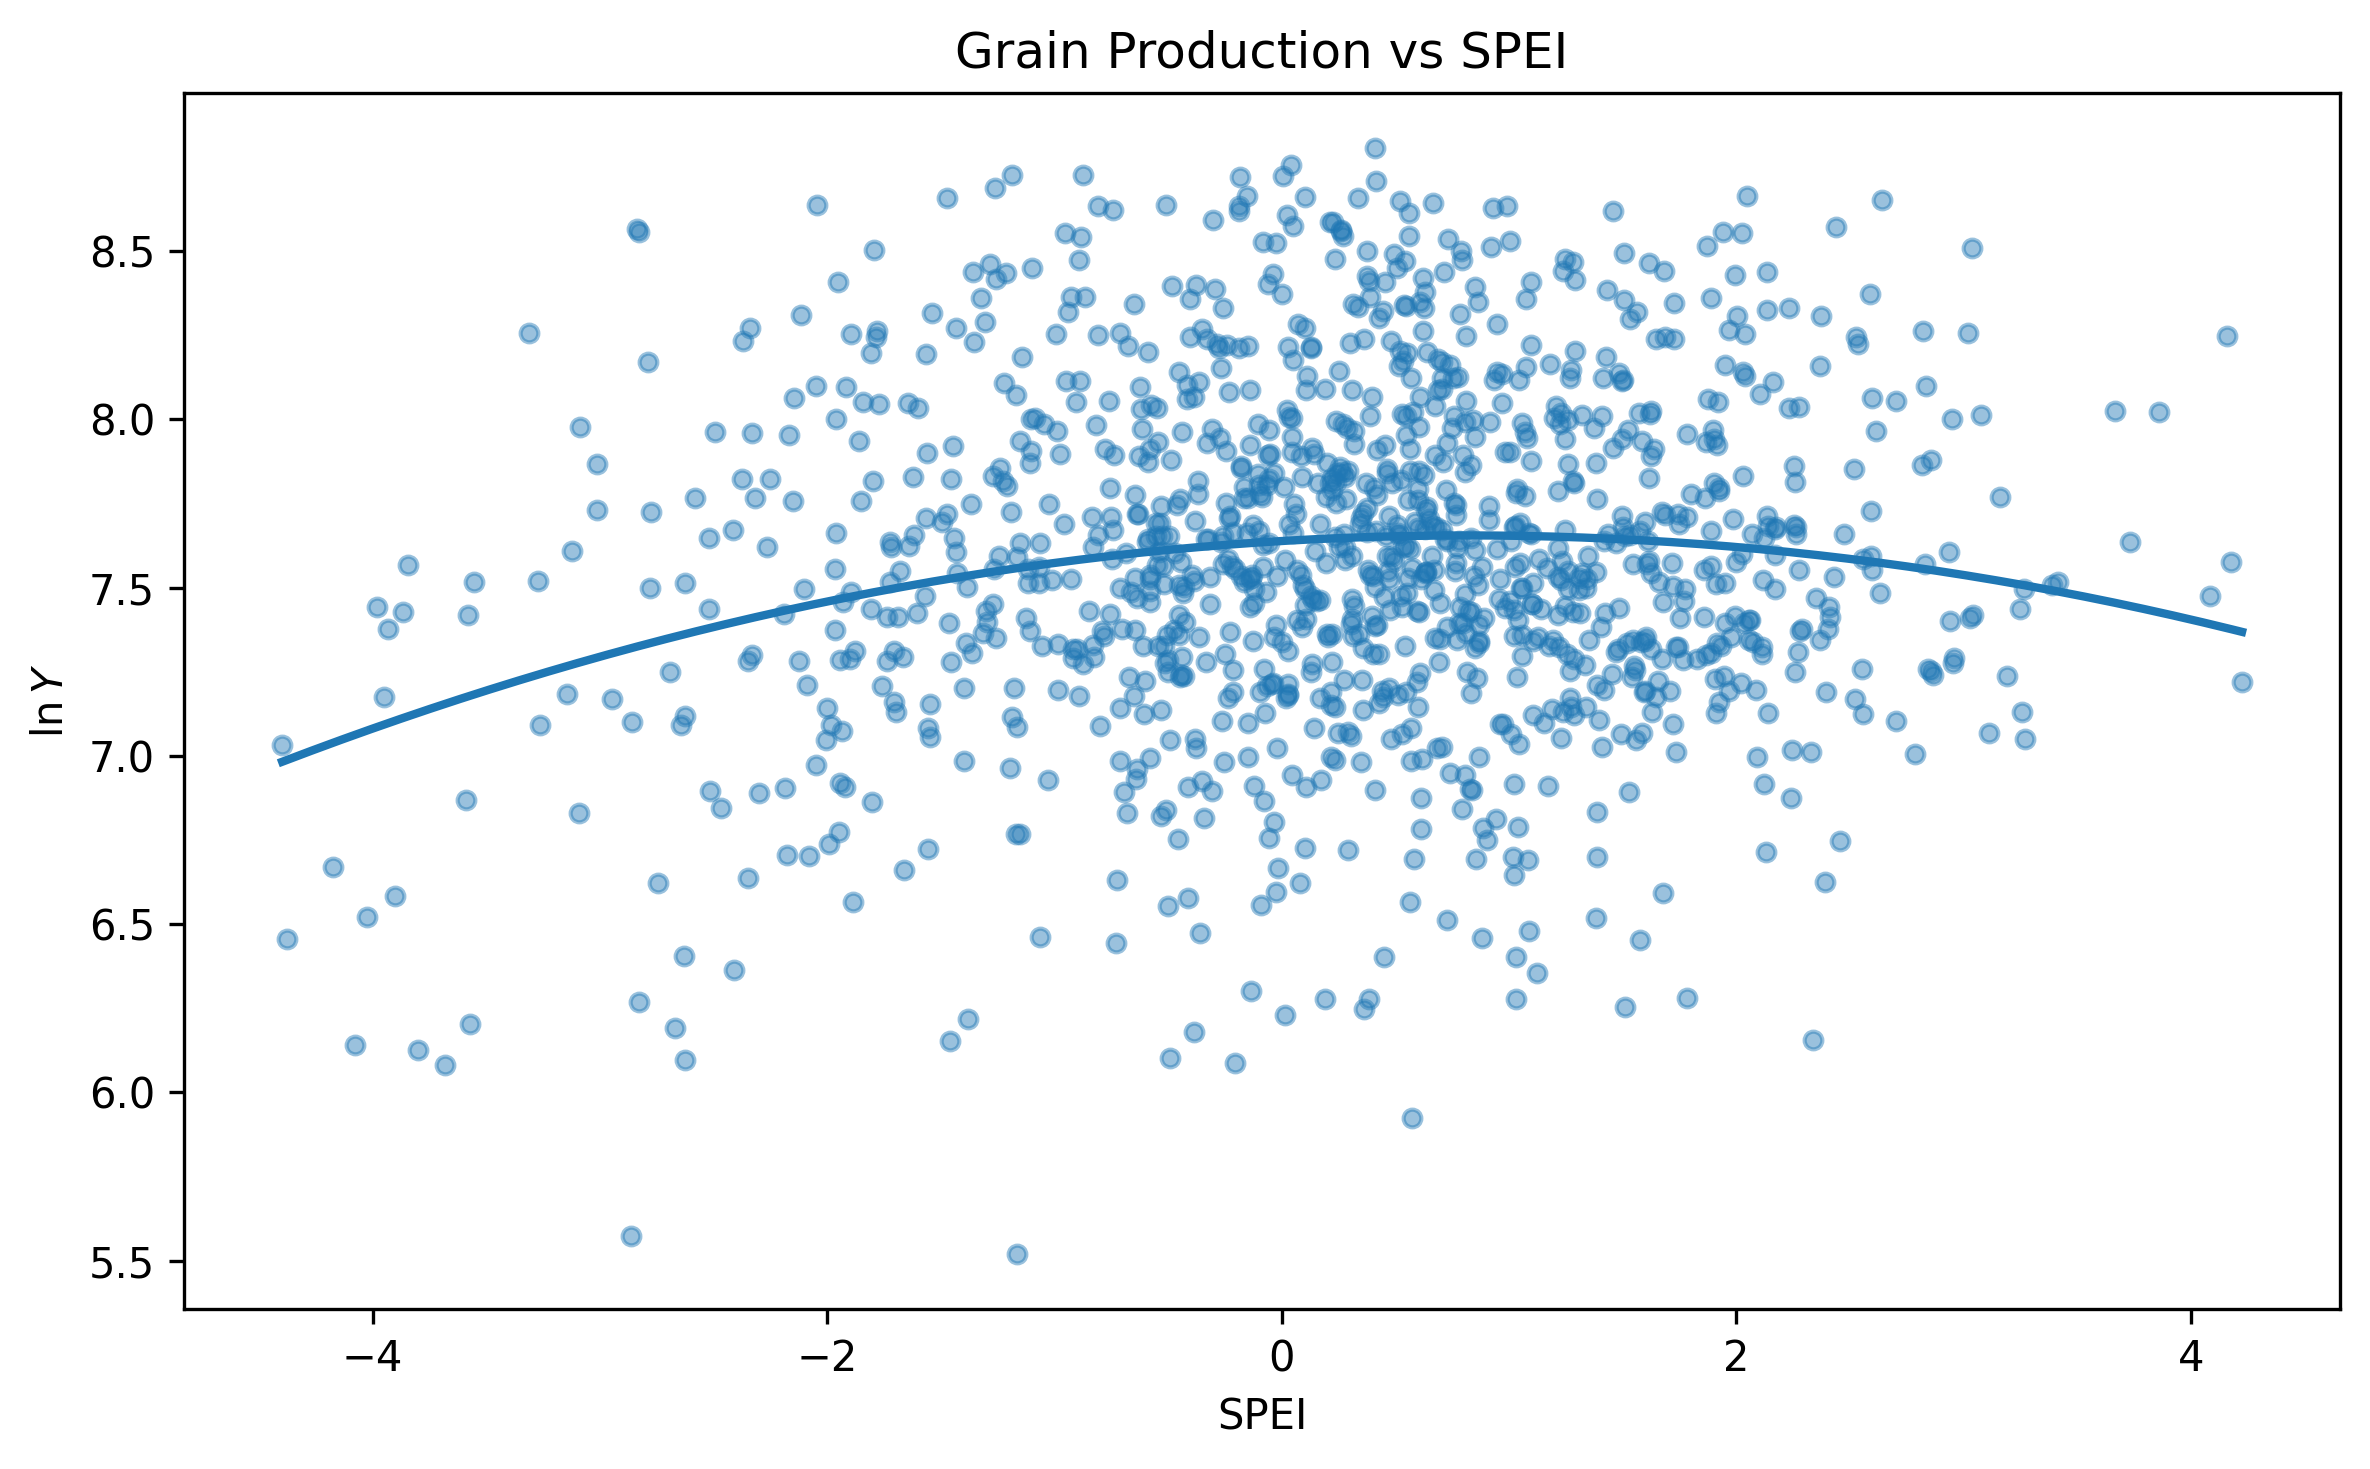
\includegraphics[width=0.75\textwidth]{spei_quadratic_fit.png}
\caption{Nonlinear relationship between SPEI and log grain production}
\end{figure}

\begin{figure}[H]
\centering
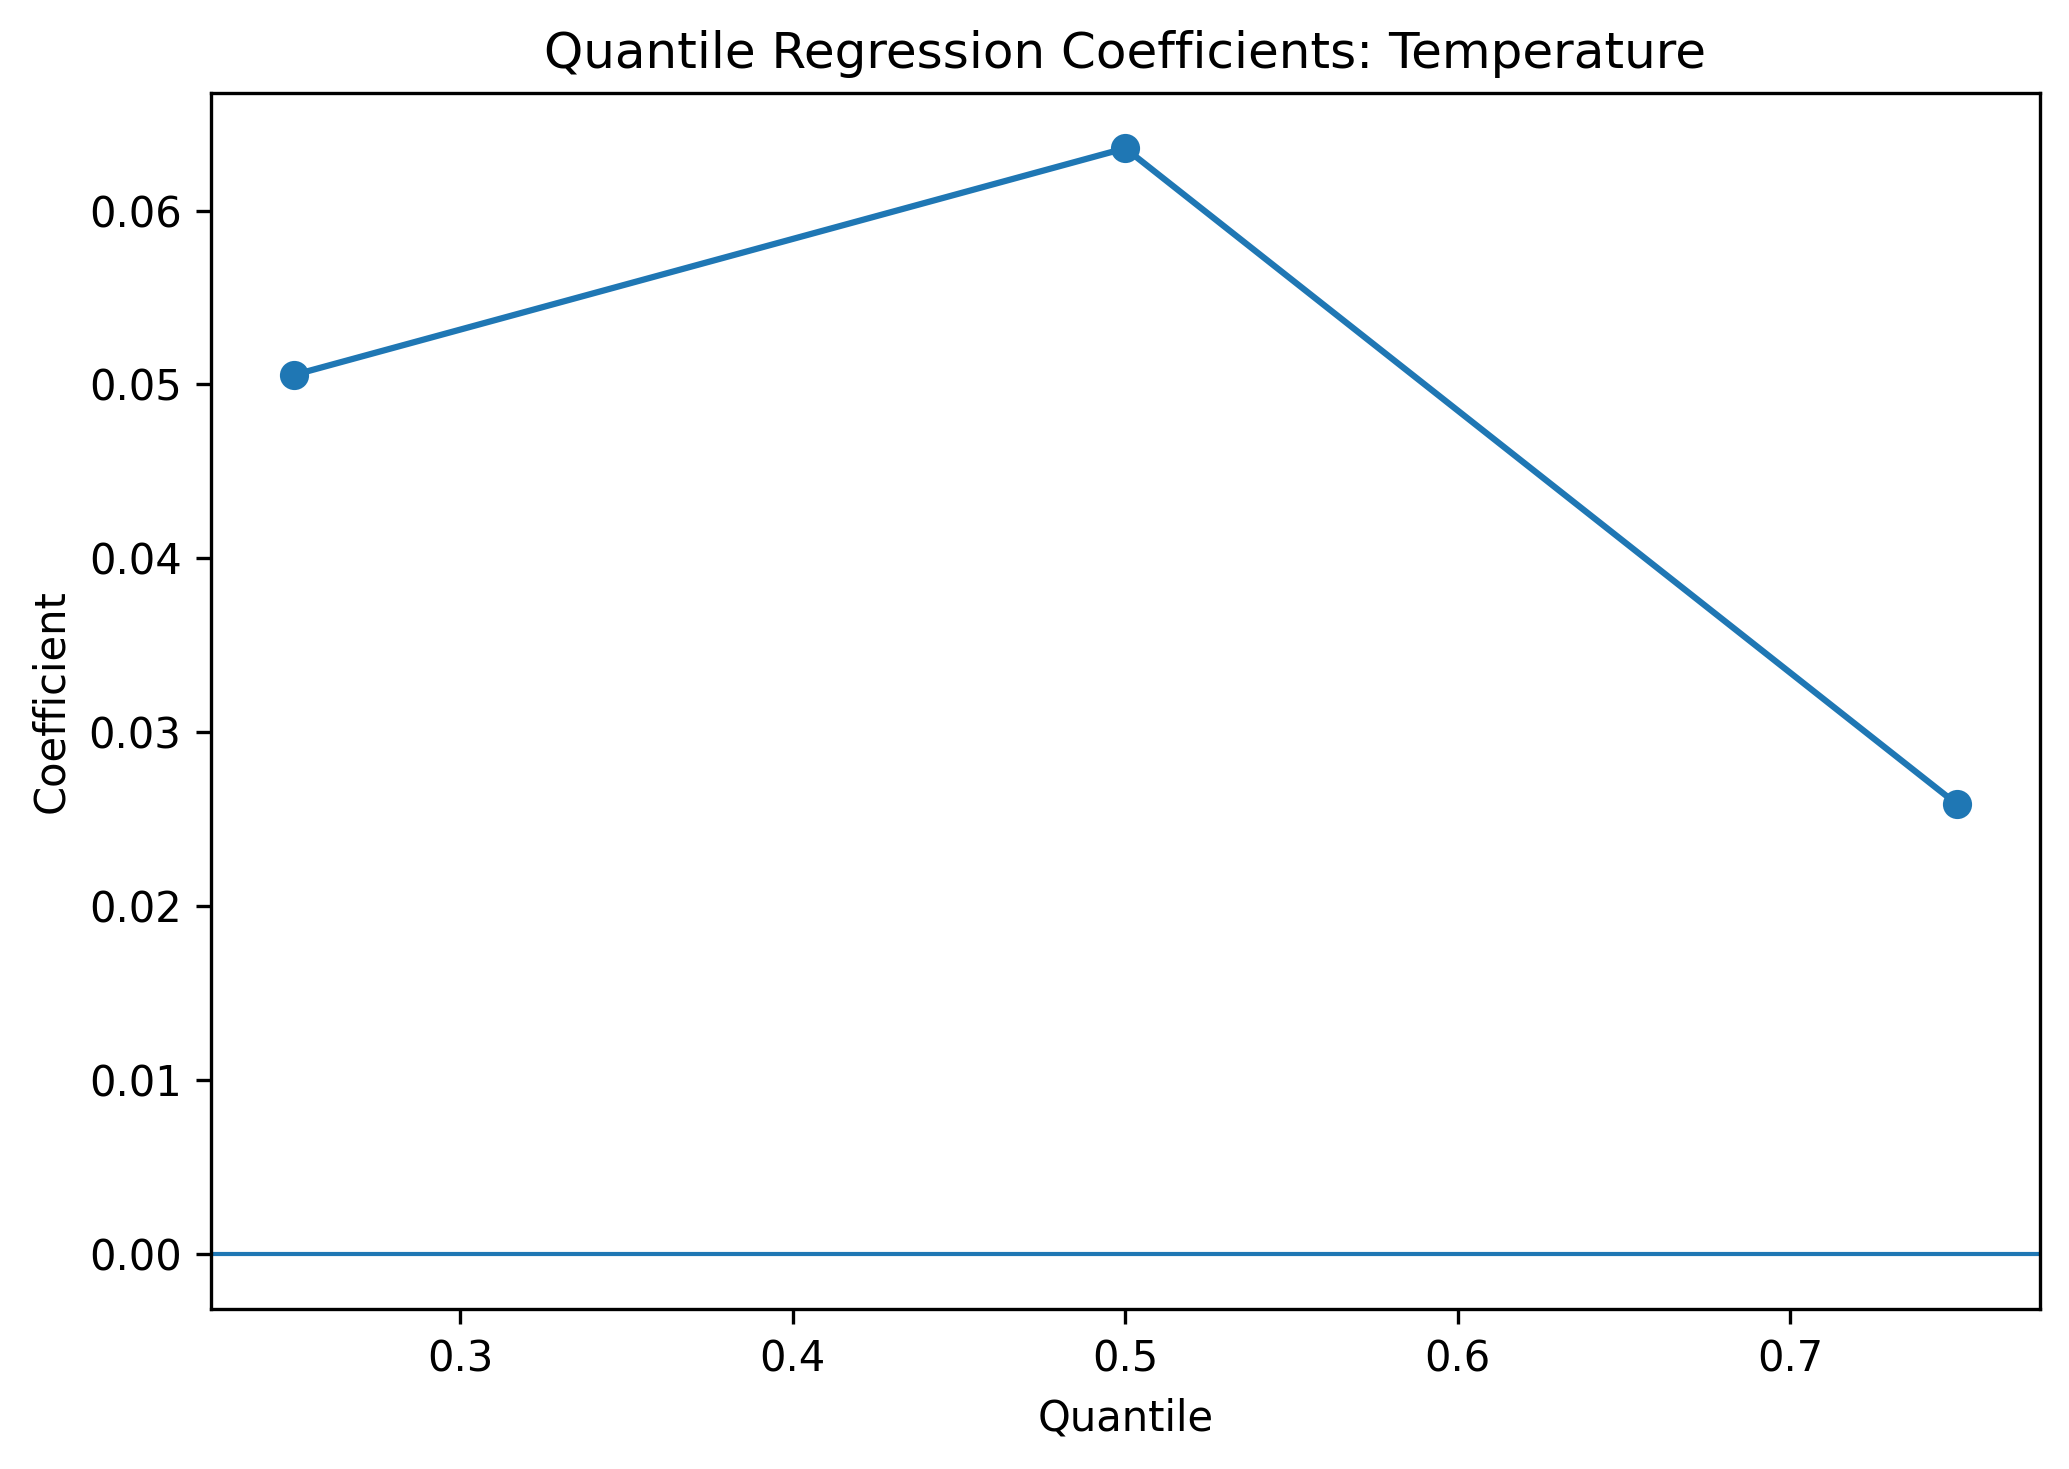
\includegraphics[width=0.75\textwidth]{quantile_temperature_coefficients.png}
\caption{Changes in growing-season average temperature coefficients across quantiles}
\end{figure}

\begin{figure}[H]
\centering
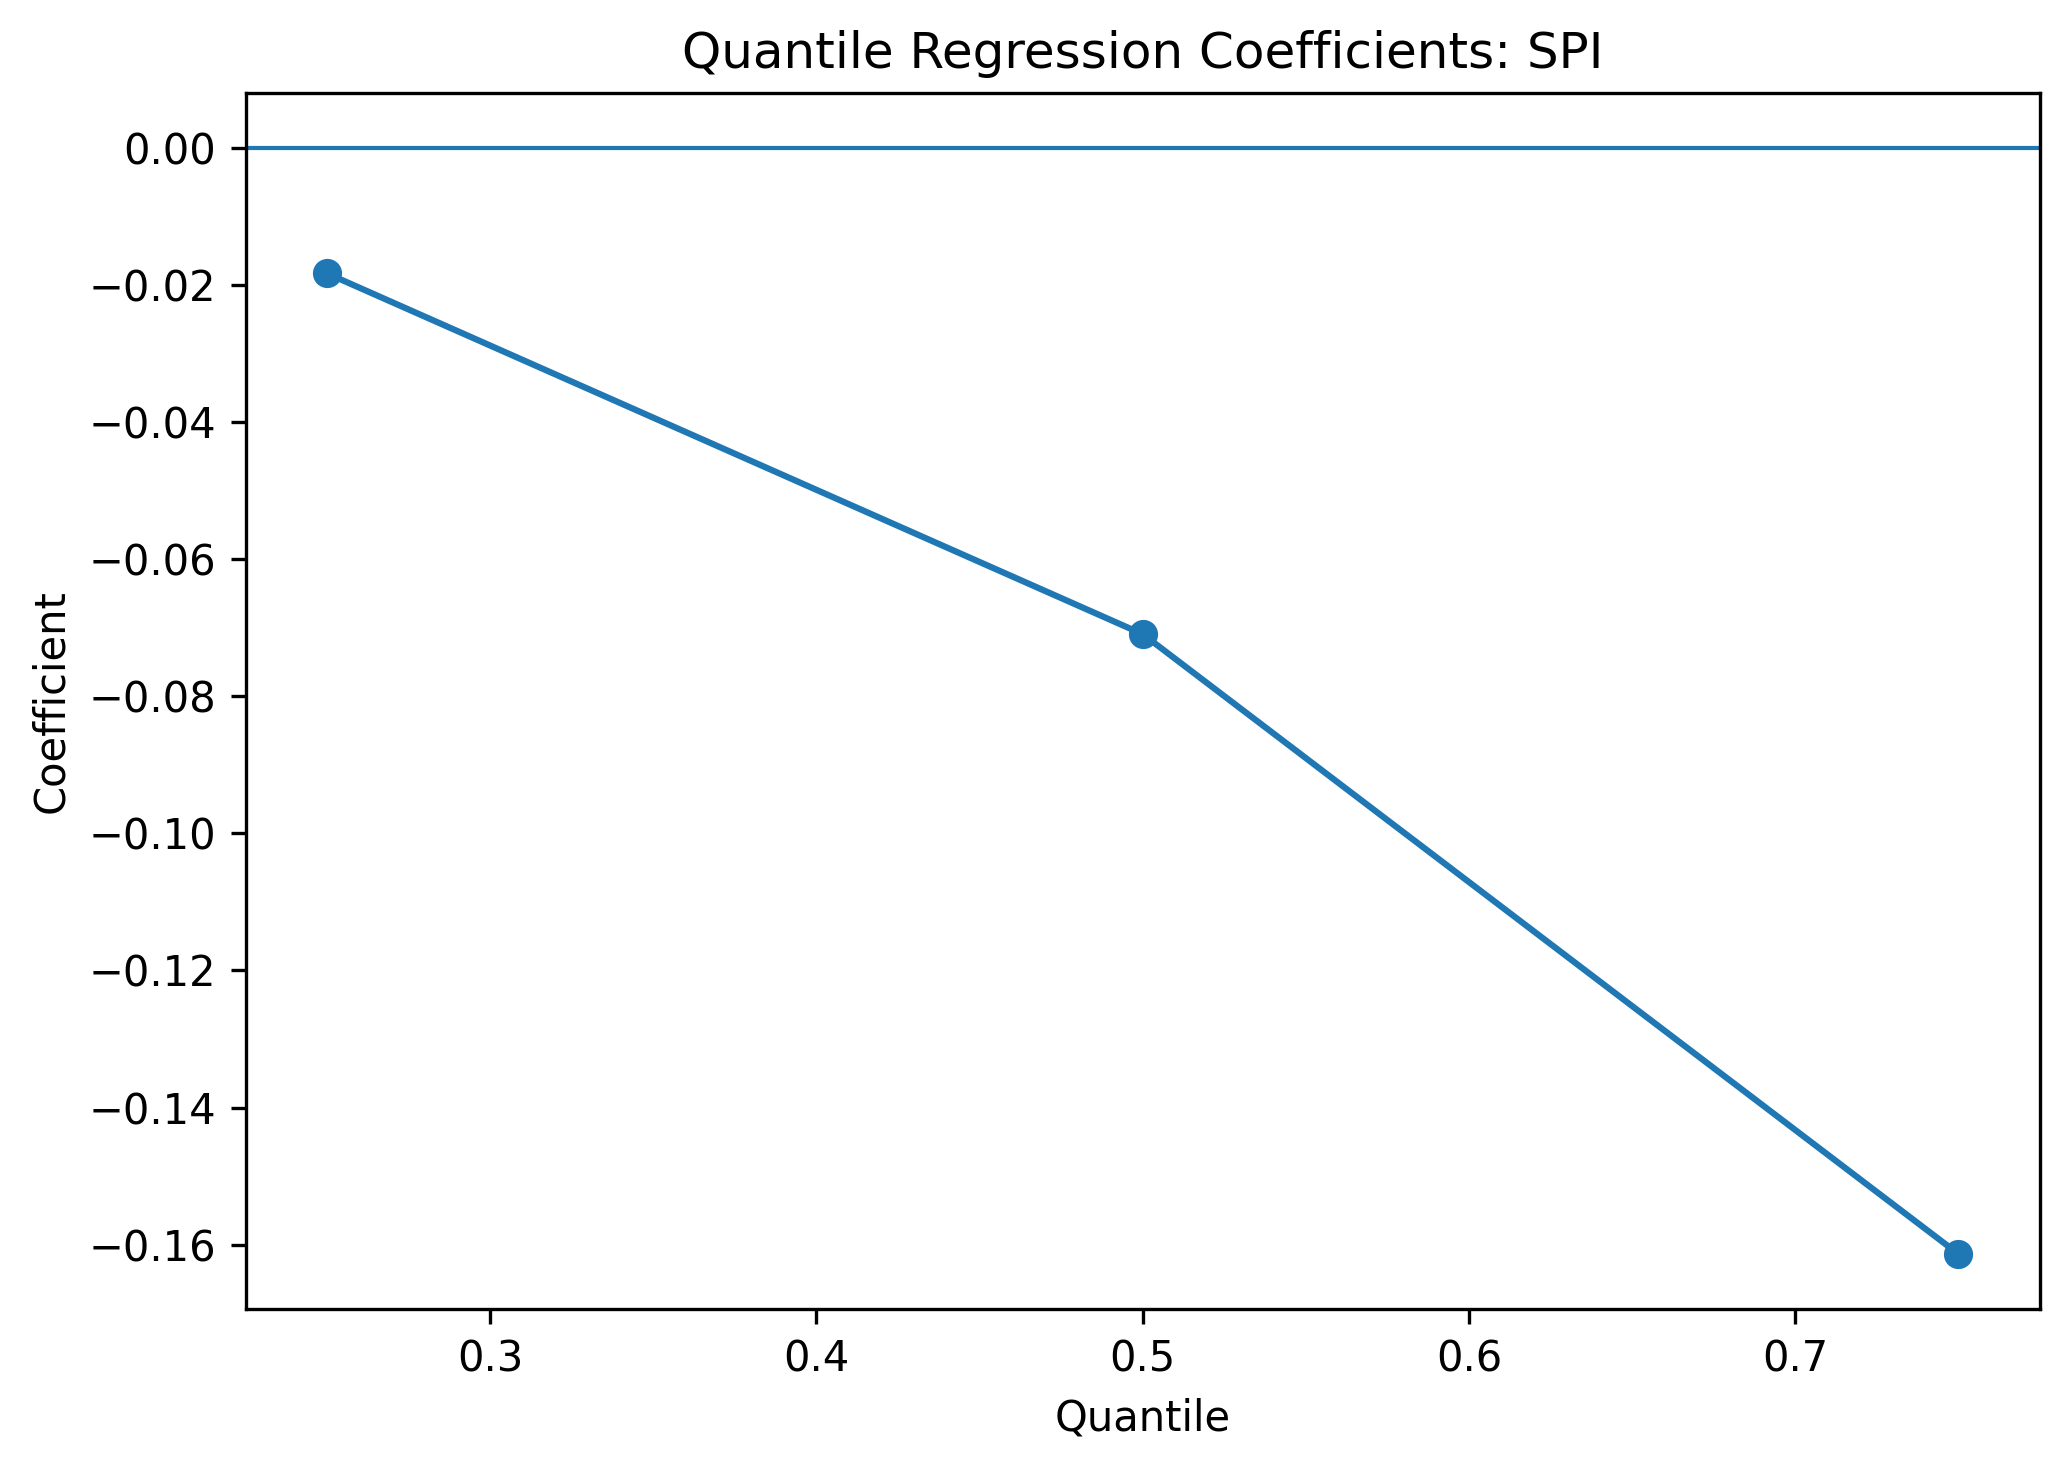
\includegraphics[width=0.75\textwidth]{quantile_spi_coefficients.png}
\caption{Changes in SPI coefficients across quantiles}
\end{figure}

\begin{figure}[H]
\centering
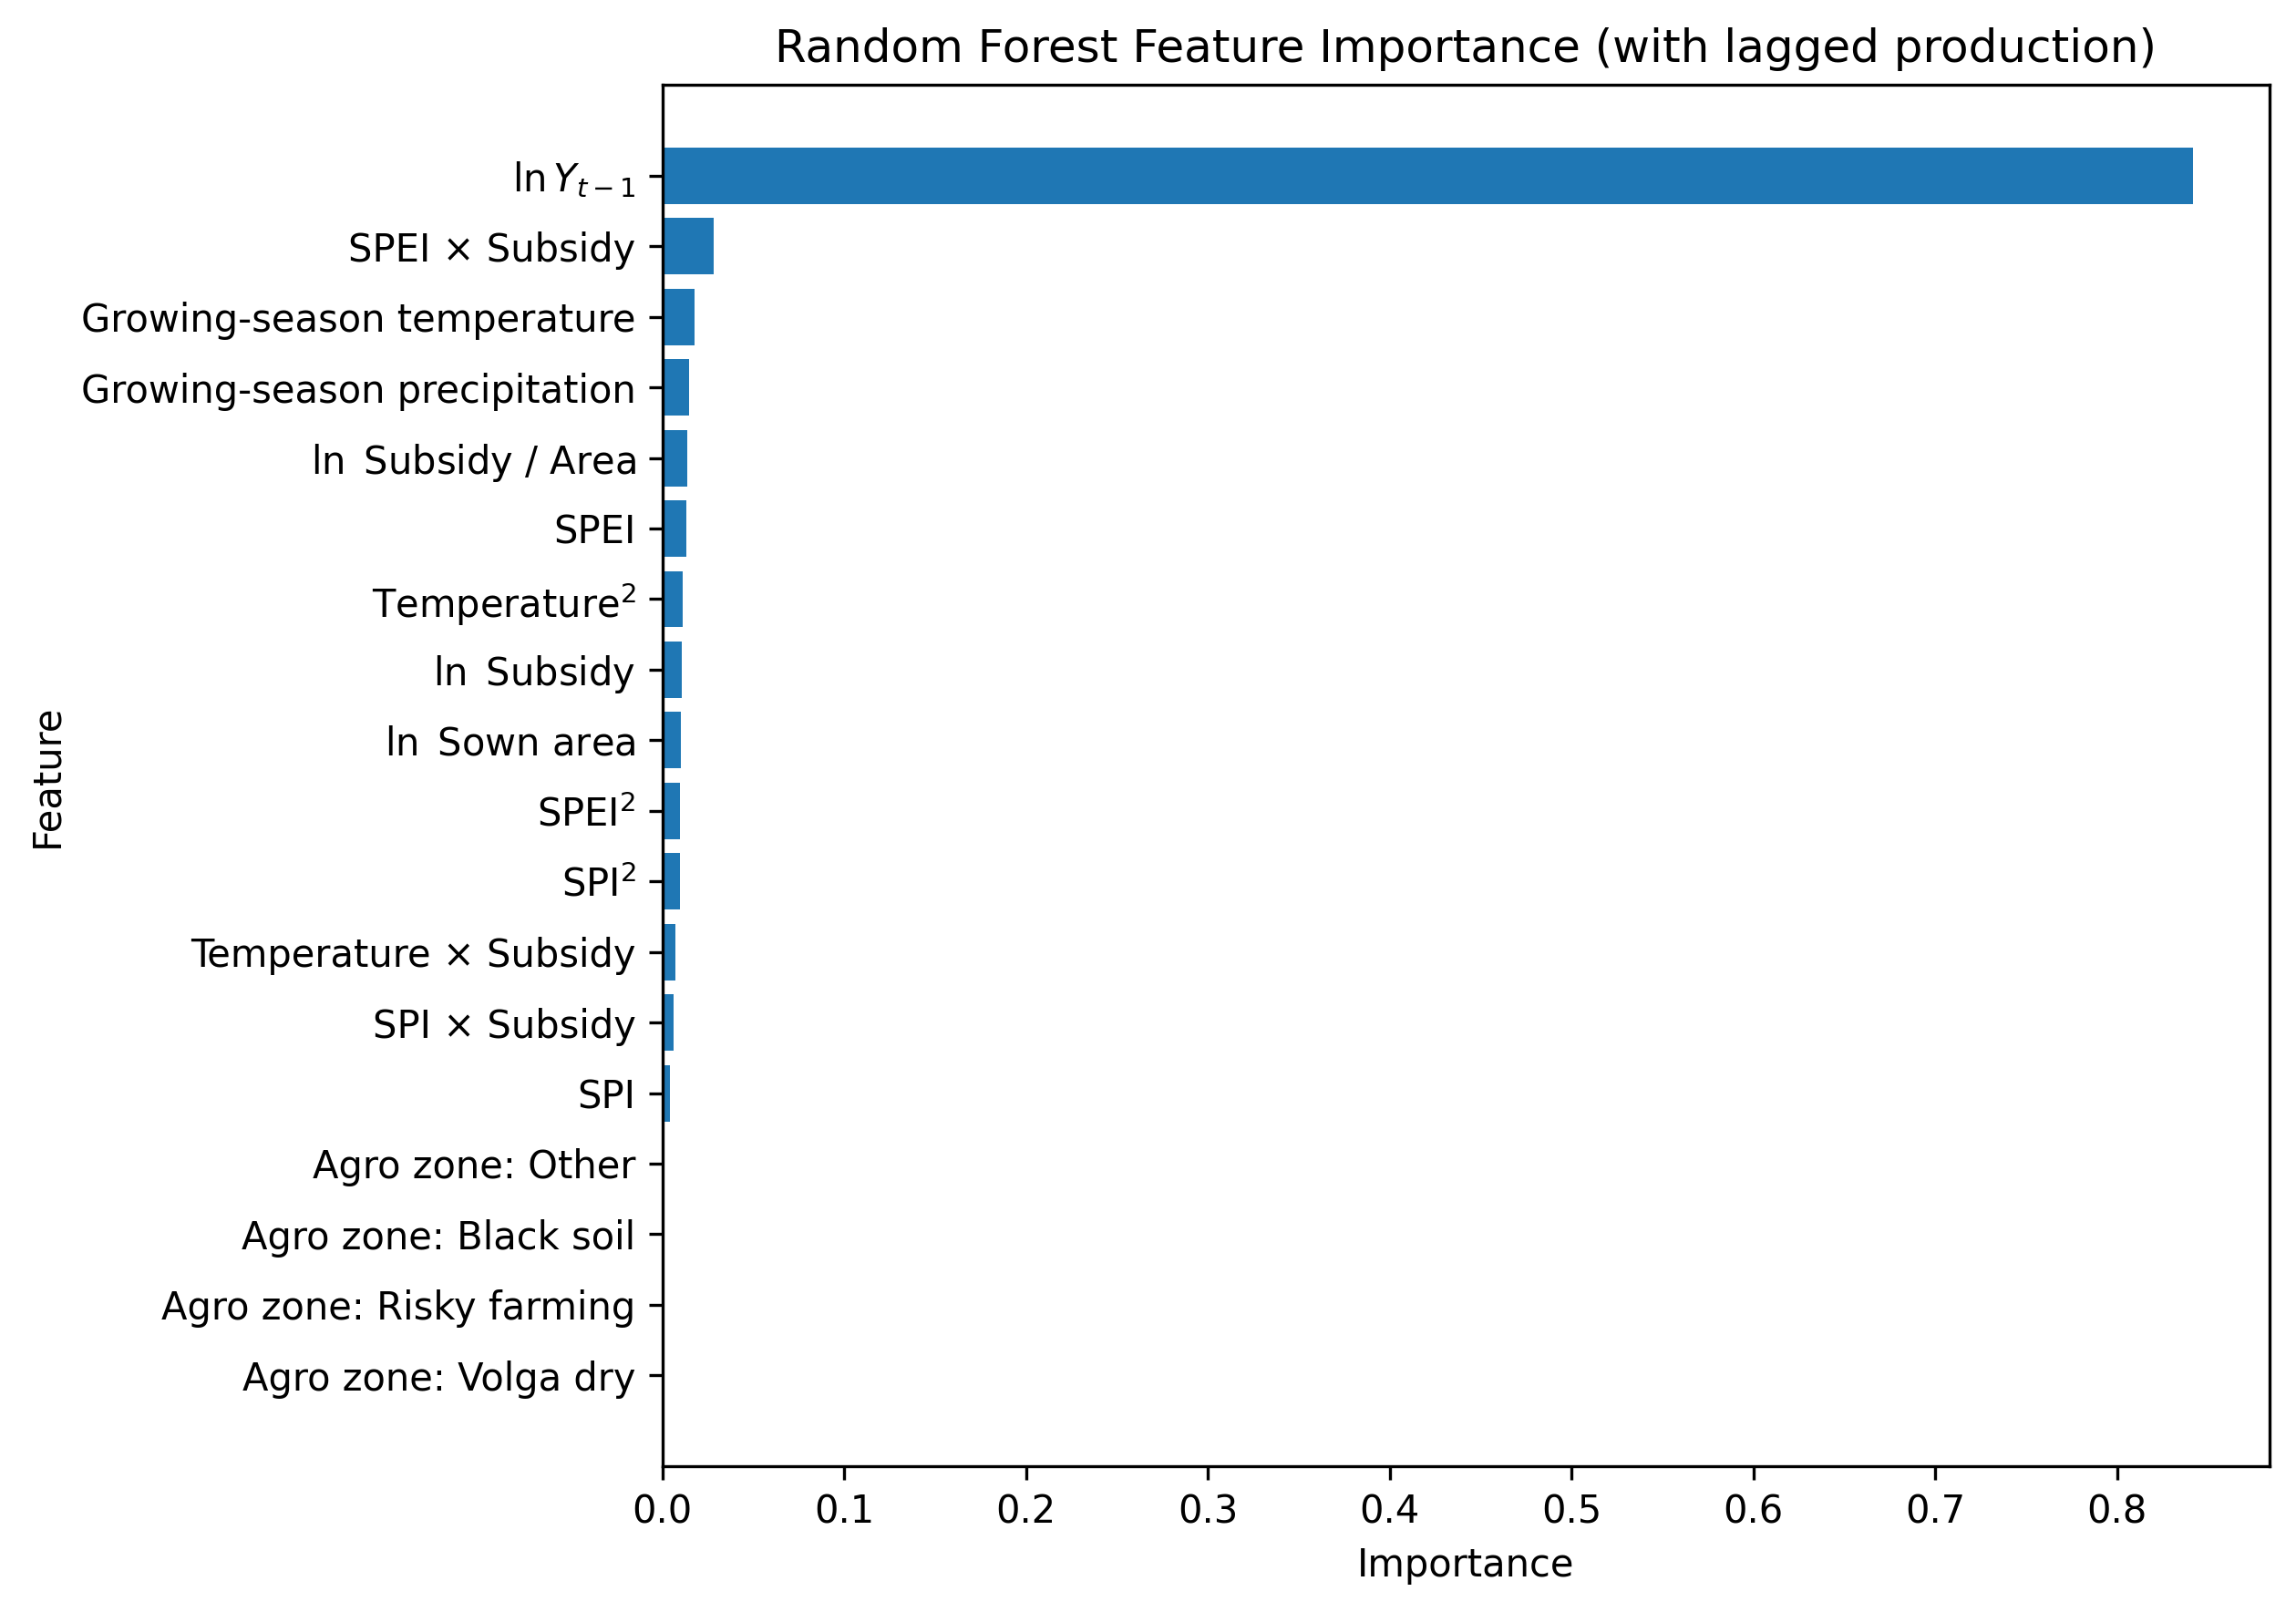
\includegraphics[width=0.85\textwidth]{rf_importance_with_lag.png}
\caption{Random forest variable importance: with lagged production}
\end{figure}

\begin{figure}[H]
\centering
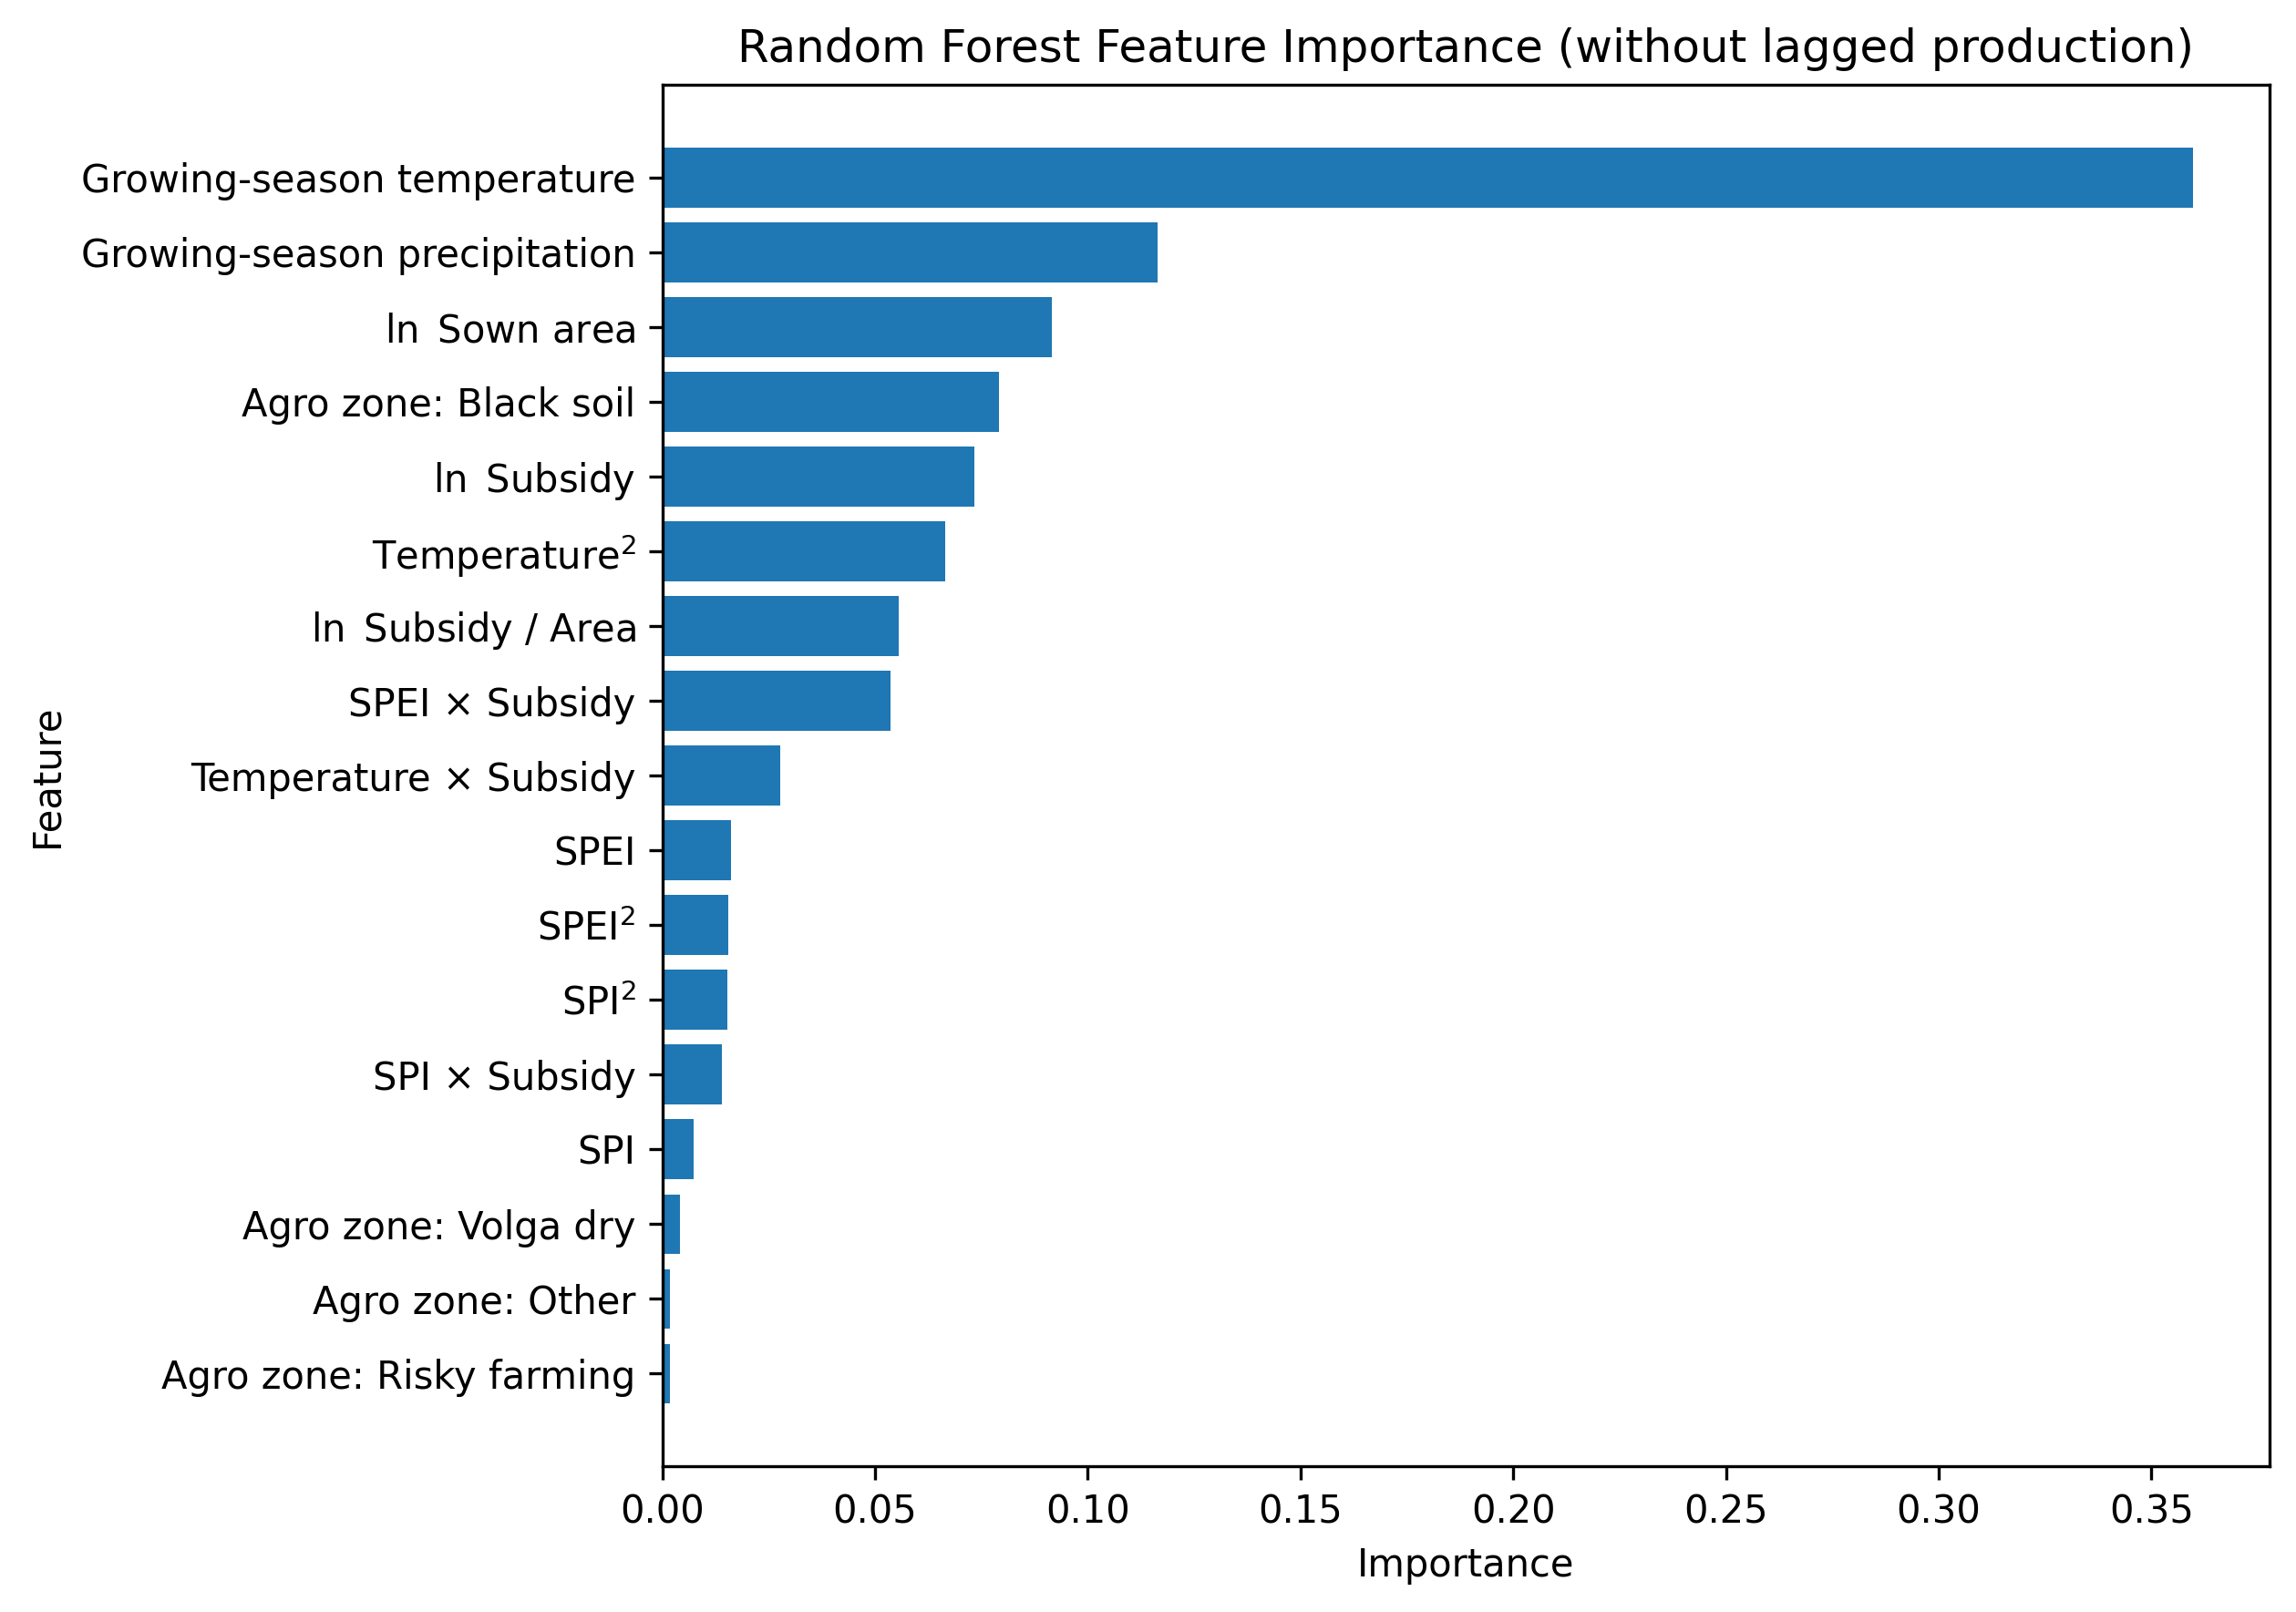
\includegraphics[width=0.85\textwidth]{rf_importance_without_lag.png}
\caption{Random forest variable importance: without lagged production}
\end{figure}

\begin{figure}[H]
\centering
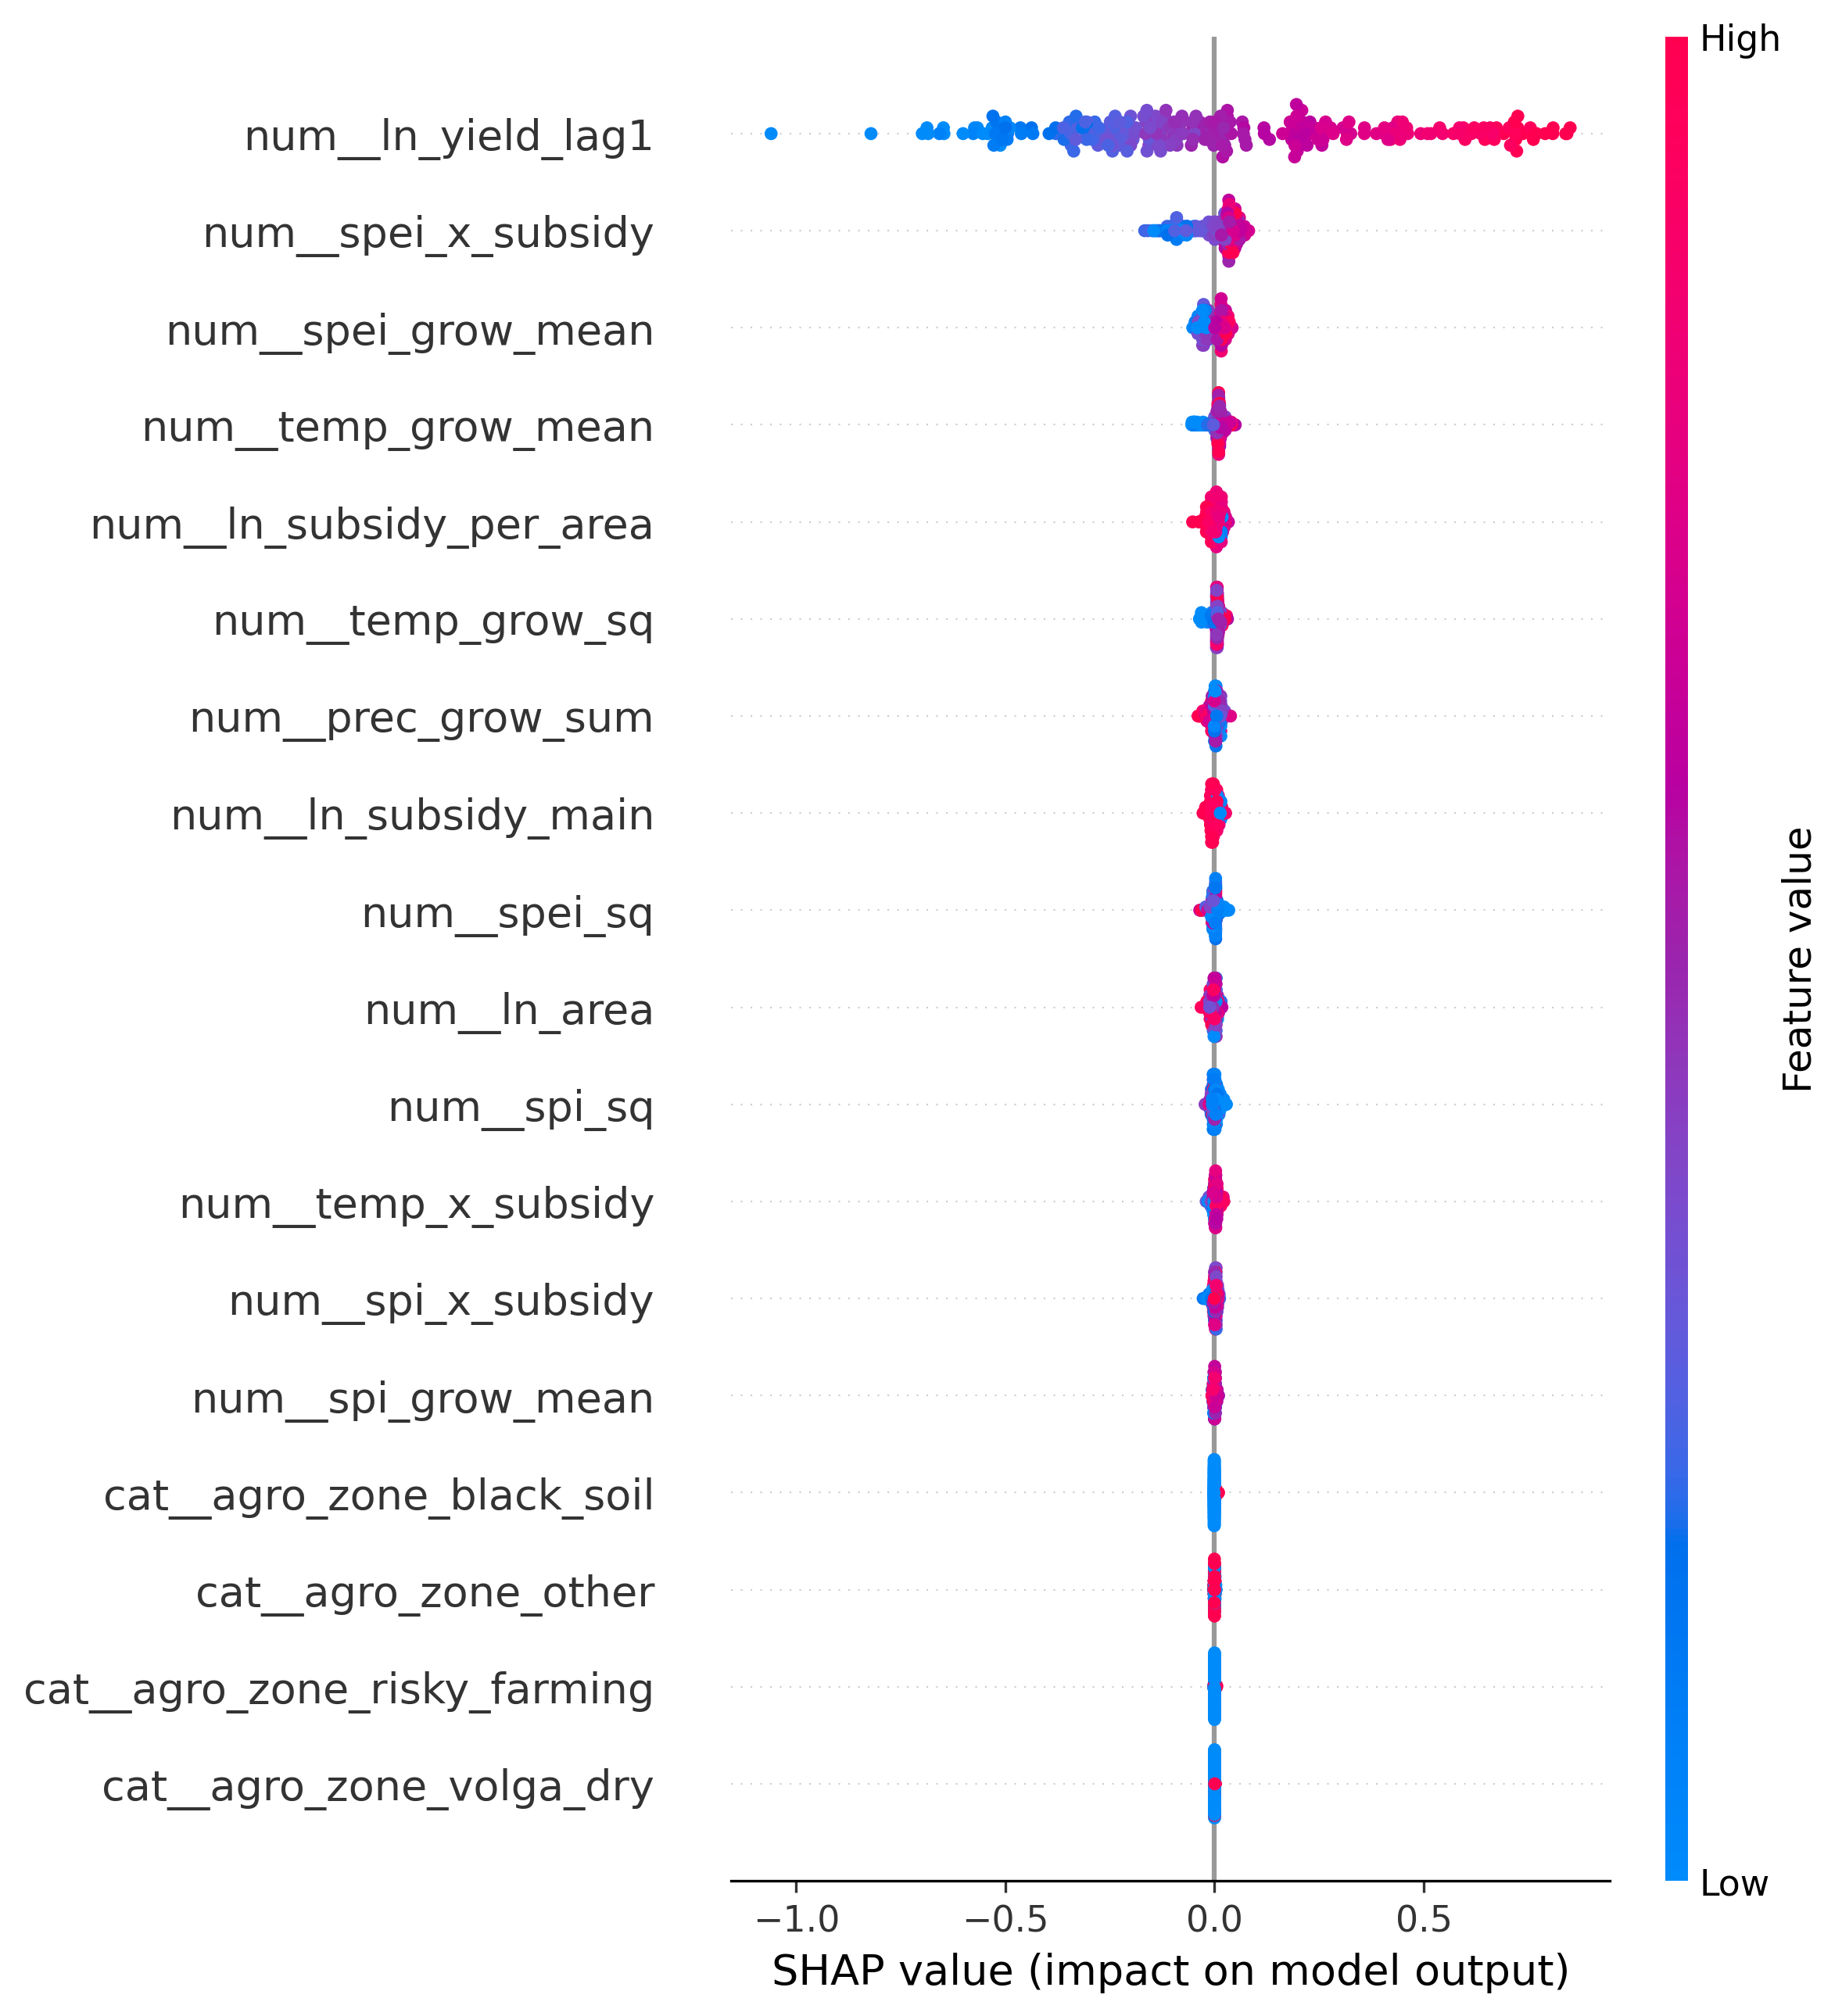
\includegraphics[width=0.85\textwidth]{shap_summary_with_lag.png}
\caption{SHAP summary plot: random forest with lagged production}
\end{figure}

\begin{figure}[H]
\centering
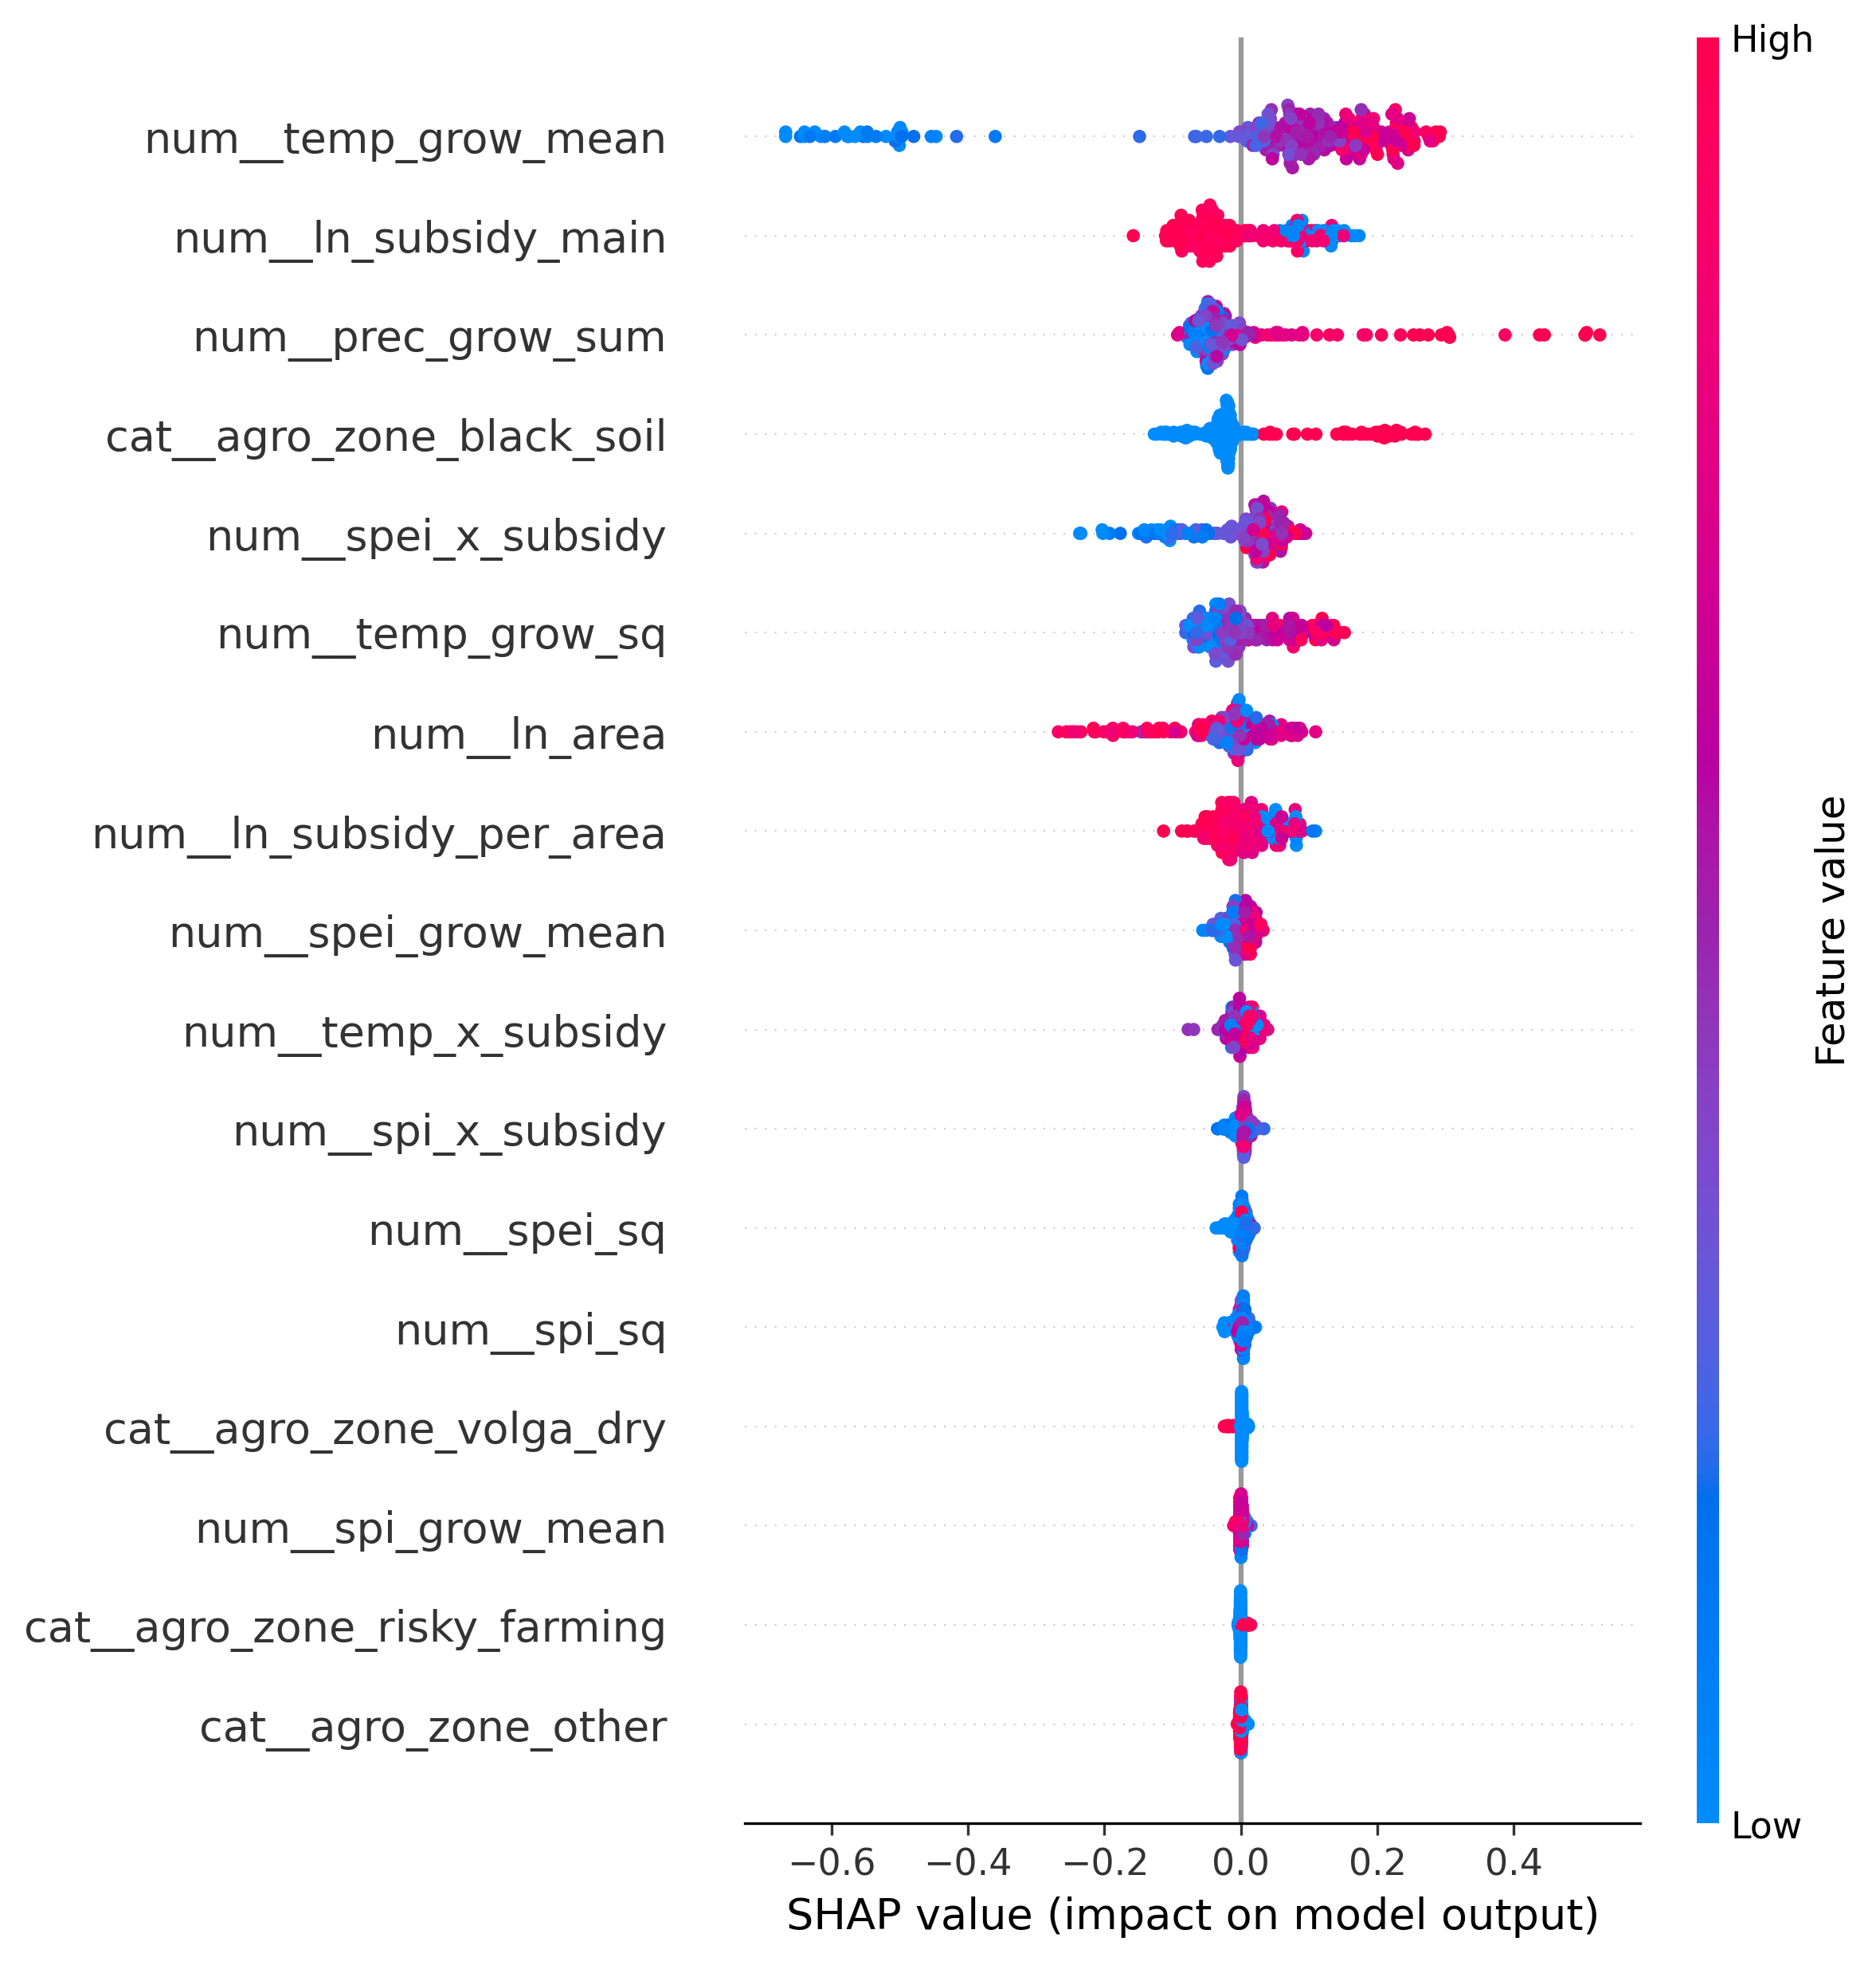
\includegraphics[width=0.85\textwidth]{shap_summary_without_lag.png}
\caption{SHAP summary plot: random forest without lagged production}
\end{figure}